% mnras_template.tex
%
% LaTeX template for creating an MNRAS paper
%
% v3.0 released 14 May 2015
% (version numbers match those of mnras.cls)
%
% Copyright (C) Royal Astronomical Society 2015
% Authors:
% Keith T. Smith (Royal Astronomical Society)

% Change log
%
% v3.0 May 2015
%    Renamed to match the new package name
%    Version number matches mnras.cls
%    A few minor tweaks to wording
% v1.0 September 2013
%    Beta testing only - never publicly released
%    First version: a simple (ish) template for creating an MNRAS paper

%%%%%%%%%%%%%%%%%%%%%%%%%%%%%%%%%%%%%%%%%%%%%%%%%%
% Basic setup. Most papers should leave these options alone.
\documentclass[a4paper,fleqn,usenatbib]{mnras}

% MNRAS is set in Times font. If you don't have this installed (most LaTeX
% installations will be fine) or prefer the old Computer Modern fonts, comment
% out the following line
\usepackage{newtxtext,newtxmath}
% Depending on your LaTeX fonts installation, you might get better results with one of these:
%\usepackage{mathptmx}
%\usepackage{txfonts}

% Use vector fonts, so it zooms properly in on-screen viewing software
% Don't change these lines unless you know what you are doing
\usepackage[T1]{fontenc}
\usepackage{ae,aecompl}


%%%%% AUTHORS - PLACE YOUR OWN PACKAGES HERE %%%%%

% Only include extra packages if you really need them. Common packages are:
\usepackage{graphicx}	% Including figure files
\usepackage{amsmath}	% Advanced maths commands
\usepackage{amssymb}	% Extra maths symbols

\usepackage[flushleft, referable]{threeparttablex} % Adding notes under tables
\usepackage{mhchem} 	% typeset chemistry symbols
% \usepackage{multicol} 	% Multi-column entries in tables
% \usepackage{natbib} % references in text to look like MNRAS/ApJ/A&A
% \usepackage{multirow} % for multirow command
\usepackage{array} % For wrapping text in cell in tables with multicolumntype




%%%%%%%%%%%%%%%%%%%%%%%%%%%%%%%%%%%%%%%%%%%%%%%%%%

%%%%% AUTHORS - PLACE YOUR OWN COMMANDS HERE %%%%%

% Please keep new commands to a minimum, and use \newcommand not \def to avoid
% overwriting existing commands. Example:
%\newcommand{\pcm}{\,cm$^{-2}$}	% per cm-squared
\defcitealias{Thomas2010}{TMJ} % TMJ alias
\newcolumntype{L}[1]{>{\raggedright\let\newline\\\arraybackslash\hspace{0pt}}m{#1}} % Multi-column entries in tables with text wrapping 
\newcommand{\bracket}[1]{[#1]} % to be able to use [] in arguments


%%%%%%%%%%%%%%%%%%%%%%%%%%%%%%%%%%%%%%%%%%%%%%%%%%

%%%%%%%%%%%%%%%%%%% TITLE PAGE %%%%%%%%%%%%%%%%%%%

% Title of the paper, and the short title which is used in the headers.
% Keep the title short and informative.
\title[An IFS study of Low-powered Radio Galaxies]{An IFS study of Low-powered Radio Galaxies}

% The list of authors, and the short list which is used in the headers.
% If you need two or more lines of authors, add an extra line using \newauthor
\author[J. Warren et al.]{
Joshua Warren,$^{1}$\thanks{Contact e-mail: \href{mailto:joshua.warren@physics.ox.ac.uk}{joshua.warren@physics.ox.ac.uk}}
Martin Bureau,$^{1}$
Bernd Hasemann,$^{2}$
Isabella Prandoni,$^{3}$ \newauthor
Francesco Santoro,$^{3}$
Robert Laing,$^{3}$
Paola Parma,$^{3}$
Hans de Ruiter$^{3}$
and \newauthor
Arturo Mignano$^{3}$
\\
$^{1}$Sub-department of Astrophysics, Department of Physics, University of Oxford, Denys Wilkinson Building, Keble Road, Oxford OX1 3RH, UK\\
$^{2}$European Southern Observatory, Karl-Schwarzschild-Str. 2, 85748 Garching b. München, Germany\\
$^{3}$INAF - Istituto di Radioastronomia, Via P. Gobetti 101, 40129 Bologna, Italy}


% These dates will be filled out by the publisher
\date{Accepted XXX. Received YYY; in original form ZZZ}

% Enter the current year, for the copyright statements etc.
\pubyear{2018}

% Don't change these lines
\begin{document}
\label{firstpage}
\pagerange{\pageref{firstpage}--\pageref{lastpage}}
\maketitle

% Abstract of the paper
\begin{abstract}
This is a simple template for authors to write new MNRAS papers.
The abstract should briefly describe the aims, methods, and main results of the paper.
It should be a single paragraph not more than 250 words (200 words for Letters).
No references should appear in the abstract.
\end{abstract}

% Select between one and six entries from the list of approved keywords.
% Don't make up new ones.
\begin{keywords}
% keyword1 -- keyword2 -- keyword3
\end{keywords}

%%%%%%%%%%%%%%%%%%%%%%%%%%%%%%%%%%%%%%%%%%%%%%%%%%

%%%%%%%%%%%%%%%%% BODY OF PAPER %%%%%%%%%%%%%%%%%%


\section{Introduction}
	\label{sec:intro}
	% There are known to be strong scaling relations between the mass of the central supermassive black-hole (SMBH) and the global properties in a given galaxy, such as velocity dispersion, the $M-\sigma$ relation \citep{Ferrarese2000, Gebhardt2000, Graham2011}; Sersic index \citep{Graham2007, Savorgnan2013}; luminosity \citep{Laor2001, McLure2001, Lauer2007, Graham2012}; etc. AGN feedback is understood to be the mechanism by which the SMBH can expand its sphere of influence to galactic scales to affect these relationship. 

	% This is generally understood to be a feedback process, where large amounts of gas within the galaxy cools, falls on the SMBH. Here the black-hole imparts energy to the gas, causing outflows (or jets) and/or thermal emission. We observe this as an Active Galactic Nuclei (AGN) which can have distinctive emission across the electromagnetic spectrum. The exact mechanisms of imparting energy still remains an open question, with much theoretical and observational work ongoing. The outflows can then effect the outer parts of the galaxy, by methods such as fountain effects \citep{}, thermal heating \citep{DeYoung2010} and shocks created by the outflows \citep{}.

	% One identifier of AGNs is a radio signature consistent with Synchrotron emission from the outflow i.e a radio galaxy (RG). These are typically categorized into one of two classes: Fanaroff-Riley (FR) I or FR II \citep{Fanaroff1974}. Of these we focus on the former since these are by far the most common mode in the local universe (possibly as far as $z \sim 1$ \citep{Rigby2008}), and so to discuss radio AGN feedback is to consider feedback from FR I sources \citep{DeYoung2010}. Indeed, while there is broad consensus \citep{Heckman1986, Baum1992} that the brightest RGs (mostly FR IIs) are caused when a massive galaxy merges with a gas rich galaxy (a wet merger) giving a plentiful fuel reservoir to the AGN \citep{Baum1992}, there is much more debate when it comes to low-powered ($P_\text{1.4 GHz} \lesssim 10^{24.5} \, \mathrm{W Hz^{-1}}$) RGs (mostly FR I). Suggestions fall into two categories: an extrapolation of radio-loud galaxies (i.e. a merger with either small gas reservoirs or low efficiency accretion onto the SMBH) or a highly efficient accretion of gas from secular origins (such as Bondi accretion of the hot X-ray component of the Inter-Stellar Medium (ISM) \citep{Allen2006} or from existing cold gas reservoirs \citep{Prandoni2010}). This project aims to add to this discussion using Integral Field Unit (IFU) observations in the visible band of nearby radio galaxies and comparing this with Atlas-3D sample \citep{Cappellari2011} as a control sample.

% More to add to intro - e.g. summery of paper 

	We refer to the combined Atlas$^\text{3D}$ and MASSIVE sample as the A+M sample.

\section{Sample Description}
	\label{sec:samp}
	The Parkes 2.7 GHz survey \citep{Ekers1989} was used as a parent sample, as it contains radio sources (down to a flux density limit of 250\,mJy at 2.7\,GHz) with an optical counterpart (with an $V$-band apparent magnitude of $m_V \le 17.0$). Host galaxies with a redshift greater than 0.03 were discarded. It is worth noting that both the radio and optical limits are apparent measurements, and as such this is not a volume-limited sample.

	\begin{table*}
		\centering
	% \begin{threeparttable}
		\caption{Key sample characteristics of the Southern Sample galaxies. Col.\,1: host galaxy name. Col.\,2: radio source name from Parkes Southern Radio Source Catalogue. We hereafter refer to the last galaxy by its PKS name only. Col.\,3: redshift. Col.\,4: National Radio Astronomy Observatory (NRAO) Very Large Array (VLA) Sky Survey (NVSS) 1.4 GHz flux density \citep{Condon1998}. Col.\,5: Two Micron All Sky Survey (2MASS) $K$-band apparent magnitude (with errors of $\pm 0.025$ mag; \citealt{Skrutskie2006}). Col.\,6: dust morphologies from (a) \citet{Govoni2000}, (b) \citet{Lauer2005}, (c) \citet{Bettoni2001}, (d) \citet{Sandage1979}, (e) \citet{Colbert2001}.}
		\label{tab:sample}
		\begin{tabular}{l c c c c l}
			\hline
			\hline
			Host galaxy	& Radio source 	& Redshift	& $S_\text{1.4\,GHz}$	& $m_K$ & Dust morphology\\
						& (PKS) 		& 			& (mJy) 			& (mag)	&\\
			\hline 
			ESO 443-G024 & 1258-321 	& 0.01703	& $1387 \pm 45$		& 8.51 & no dust\tnote{a}	\\ 
			IC 1459 	& 2254-367 		& 0.00565 	& $1280 \pm 45$		& 6.81 & dust lane\tnote{b}	\\
			IC 1531 	& 0007-325 		& 0.02553 	& \leavevmode\phantom{0}$388 \pm 12$		& 9.55 & --					\\
			IC 4296		& 1333-\leavevmode\phantom{0}33 		& 0.01248 	& $1342 \pm 41$		& 7.50 & edge-on disc\tnote{b} \\
			NGC 612 	& 0131-\leavevmode\phantom{0}36 		& 0.02954 	& \leavevmode\phantom{0}$585 \pm 18$		& 9.58 & dust lane\tnote{c}	\\
			NGC 1316 	& 0320-\leavevmode\phantom{0}37 & 0.00591 	& \leavevmode\phantom{0}$255 \pm 10$		& 5.59 & dust patches\tnote{b} \\
			NGC 1399 	& 0336-\leavevmode\phantom{0}35 & 0.00472 	& \leavevmode\phantom{0}$209 \pm \leavevmode\phantom{0}7$	& 6.31 & no dust\tnote{b}	\\
			NGC 3100 	& 0958-314 		& 0.00879 	& \leavevmode\phantom{0}$530 \pm 16$		& 8.08 & dust lane\tnote{d}	\\
			NGC 3557 	& 1107-372 		& 0.01016 	& \leavevmode\phantom{0}$484 \pm 16$		& 7.20 & face-on disc\tnote{b}\\
			NGC 7075 	& 2128-388 		& 0.01819 	& \leavevmode\phantom{0}$837 \pm 28$		& 9.56 & --					\\
			--			& 0718-\leavevmode\phantom{0}34 		& 0.02897 	& $1119 \pm 41$		& 9.97 & dust patches\tnote{e} \\
			\hline
			\hline
		\end{tabular}
	% 	\begin{tablenotes}
	% 	\footnotesize
	% 	\note Col.\,1: host galaxy name. Col.\,2: radio source name from Parkes Southern Radio Source Catalogue. Col.\,3: redshift. Col.\,4: National Radio Astronomy Observatory (NRAO) Very Large Array (VLA) Sky Survey (NVSS) 1.4 GHz flux density \citep{Condon1998}. Col.\,5: Two Micron All Sky Survey (2MASS) $K$-band apparent magnitude (with errors of $\pm 0.025$ mag; \citealt{Skrutskie2006}). Col.\,6: dust morphologies from (a) \citet{Govoni2000}, (b) \citet{Lauer2005}, (c) \citet{Bettoni2001}, (d) \citet{Sandage1979}, (e) \citet{Colbert2001}. 
	% 	\item We hereafter refer to the last galaxy by its PKS name only.
	% 	\end{tablenotes}
	% \end{threeparttable}
	\end{table*}

	These criteria lead to a sample of 11 galaxies hereafter referred to as the Southern Sample. The key observed characteristics are summarised in Table \ref{tab:sample}.
	%, while the derived characteristics are listed in Table \ref{tab:sampleDerived}. 
	All galaxies have a FR I radio morphology according to the \citet{Fanaroff1974} scheme; the bulk of the radio emission is centrally-concentrated, as opposed to the FR II morphology where the brightest points are at the ends of the radio lobes. 
	
	The sample was initially observed with the Atacama Pathfinder Experiment \citep[APEX; ][]{Gusten2006}, with detections claimed for the \ce{^{12}CO(2-1)} transition for all galaxies. Some galaxies had extremely large line widths (up to a full-width half-maximum of $904 \, \mathrm{km \, s^{-1}}$ for IC 4296), but most showed a flat or double-horn spectrum indicative of ordered rotation \citep{Prandoni2012}.


\section{Observing strategy and Data Reduction}
	\label{sec:obs}
	The sample was observed with the Visible Multi-Object Spectrograph (VIMOS), mounted on UT3 on the VLT in Paranal \citep{LeFevre2003}. All observations were taken with a spatial sampling of $0\farcs67$, using the high-resolution blue grism yielding a wavelength range of 3700-5520\,\AA\ with a spectral resolution of 1440 and sampling of 0.71\,\AA\,$\mathrm{pix^{-1}}$. Each object was observed with a total integration time of $\approx 100$\,min on-source, equally spread over three observing blocks (OBs). Each OB also contained all the necessary observation for standard IFS data reduction. 

	VIMOS has several well-known though poorly-understood technical issues. These include several low transmission (bad) fibres, strong flexure, contamination from adjacent spectra on the CCD (cross-talk) and large differences in sensitivity across its 4 quadrants. To address these issues, we adopted a data-reduction pipeline produced using \textsc{Py3D}, a suite of programs based on the \textsc{python} versions of those developed for the Calar Alto Legacy Integral Field spectroscopy Area survey \citep[CALIFA;][]{Sanchez2012, Husemann2013} but later updated for VIMOS by \citet{Husemann2014}. \textsc{Py3D} applies all standard IFS data-reductions steps: bias subtraction, spectrum identification, flatfielding and wavelength calibration. In addition, the data was flux calibrated using publicly available observations of the spectro-photometric standard star Feige 110 provided by ESO. All steps include methods to account for the bad fibres, flexure and cross-talk within VIMOS. 

	Following this, we noted that the cubes where still not properly calibrated. Three main issues remain: the quadrants have different intensities, clearly showing uncorrected throughput differences; diagonal intensity stripes are present in the reconstructed images at all wavelengths; and spectral features are observed \citep{Jullo2008} that are visually similar to fringe patterns caused by interference within the CCD between incident light and light reflected from the interfaces between layers of the CCD materials. \citet{Lagerholm2012} present ad-hoc methods to correct for these issues, which we here adopt. These additional steps mean that the datacubes are not perfectly flux-calibrated, but all the corrections are multiplicative and thus will not effect equivalent width or line ratio measurements. From comparisons to the MUSE data (see Section \ref{subsec:MUSE}), we then estimate the flux calibration of the resulting datacubes. 

	These method are not completely effective and some artefacts are still present in the data, however in most cases the data is of sufficient quality for our purposes. For the worst effected datacubes, we have archival observations (see Section \ref{subsec:MUSE}).

	The variance spectra are propagated throughout the data-reduction pipeline (including these ad-hoc corrections) and are square-rooted at this point, to be used as noise inputs in the following analyses (see Section \ref{sec:analysis}).


	\subsection{MUSE Archival Data}
		\label{subsec:MUSE}
		Four of the sample galaxies are in the Multi-unit Spectroscopic Explorer (MUSE) archive: IC 1459, IC 4296, NGC 1316 and NGC 1399. We include these in our analysis as they have better (spatial and spectral) resolution and sampling, a larger field-of-view and larger wavelength range than the VIMOS data. 

		We used the pre-reduced (Phase 3) datacubes from ESO. These were generally of sufficient quality for our purpose, except in both IC 1459 and IC 4296 the sky appears to have been over-subtracted. To remove this over-subtraction, we developed our own pseudo-sky subtraction routine. A median spectrum was taken from four $20 \times 20$\,spaxel regions, one in from each spatial corner of the ESO reduced cube. After checking that no stellar continuum could be fit to the medium sky spectrum (i.e.\ that very little light from the galaxy is contaminating the pseudo-sky regions), this median sky spectrum was subtracted from each spaxel in the cube. 

		Finally, we trimmed all the MUSE cubes to the central $30\arcsec \times 30\arcsec$ ($150 \times 150$\,spaxels) only, to (a) avoid the regions used for the pseudo-sky spectrum and (b) reduce the computing resources required for spatial binning (see Section \ref{sec:analysis}). In any case, the bins would likely be so large in the outer parts as to be effectively useless.

\section{Data Analysis}
	\label{sec:analysis}
	From this point on, the VIMOS and MUSE datasets are treated almost identically, the only difference (other than the different spectral ranges and resolutions) being that the MUSE datacubes are spatially binned to a higher signal-to-noise ratio (S/N) using Voronoi binning\footnote{http://www-astro.physics.ox.ac.uk/~mxc/software/} \citep{Cappellari2003}. For our purposes, we define the `signal' and `noise' of each spaxel as the median value of its spectrum and noise spectrum, respectively. We require a S/N of 30 for all VIMOS datacubes and 50 for the IC 1459 and IC 4296 MUSE datacubes. The NGC 1316 and NGC 1399 MUSE datacubes were binned to a S/N of 50 for the analysis of the stellar kinematics and 100 for the analysis of the emission line kinematics and stellar populations.

	Next we implement a routine to find optimal initial guesses of the redshift and velocity dispersion for each galaxy, to be used when fitting individual bins, by means of iterative fits to the spatially collapsed (i.e. summed across both spatial dimensions of the datacube) spectrum. We use the penalized-fitting (\textsc{pPXF}) routine\footnote{http://www-astro.physics.ox.ac.uk/~mxc/software/} of \citet{Cappellari2004} and \citet{Cappellari2016a} with the Medium-resolution Issac Newton Telescope (INT) Library of Empirical Spectra (MILES) library \citep{Sanchez-Blazquez2006, Falcon-Barroso2011a} to find the best-fitting line-of-sight velocity distribution (LOSVD; as parametrised by the Gaussian parameters $v$, the mean velocity and $\sigma$, the velocity dispersion). The final mean velocity of a given galaxy, is used as its precise spectroscopic redshift and is given in Table \ref{tab:sample}. Beyond this point, each bin is analysed independently.

	\subsection{Stellar Kinematics}
		\label{subsec:starKin}
		Each bin is fit independently again using \textsc{pPXF} with the MILES library. For the fit, regions around potential emission lines (list below) are masked, and a fourth order polynomial additive continuum correction is used. A Monte--Carlo (MC) estimate of the uncertainties is used. 

	\subsection{Ionized Gas Distribution and Kinematics}
		\label{subsec:EmissionLines}
		We fit the ionized gas fluxes and kinematics for the emission lines [\ion{O}{ii}], H$\delta$, H$\gamma$, H$\beta$, [\ion{O}{iii}], [\ion{N}{I}], [\ion{O}{i}], [\ion{N}{ii}], H$\alpha$ and [\ion{S}{ii}] using Gaussian templates. This independently fits emission lines from the interstellar medium (ISM), with a single LOSVDs (again parametrised by the Gaussian parameters $v$, the mean velocity and $\sigma$, the velocity dispersion), independently of the stellar kinematics. In the cases of the [\ion{O}{iii}], [\ion{O}{i}] and [\ion{N}{ii}] doublets, the two components of the doublets are fit with a fixed flux ratio of 1:0.34. The [\ion{N}{i}] doublet has a fixed ratio of 1:0.65 \citep{Safier1992}. The two components of the [\ion{O}{ii}] and [\ion{S}{ii}] doublets are fit independently. To minimize template mismatch, whereby emission lines are erroneously fitted to the edges of badly modeled and thus subtracted absorption features, we follow the method set out in \citet{Sarzi2005}, whereby the stellar component is first fitted as above with masked potential emission line regions, followed by the unmasking and fitting of the [\ion{O}{iii}] doublet which sets the kinematics for all the emission lines and finally the amplitude of the remaining emission lines. %Some of the forbidden emission lines have the ratio of their amplitudes fixed (see Table \ref{tab:EmissionLine}, Col.\,4).



		% \begin{table}
	 % 		% \centering
	 % 	% \begin{threeparttable}
	 % 		\caption{Emission lines considered in the \textsc{pPXF} fits. Col\,1: Emission line name. Col\,2: Emission line rest-frame wavelength. Col\,3: Doublet rest-frame wavelength for forbidden lines. Col\,4: The fixed ratio of the amplitudes of the lines within a doublet. `Free' indicates the amplitudes of both doublet constituents are fit independently of each other.}
	 % 		\label{tab:EmissionLine}
	 % 		\begin{tabular}{l c c c}
	 % 		\hline
	 % 		\hline
	 % 		Emission & Rest-frame & Doublet rest-frame & Amplitude  \\
	 % 		Line & wavelength & wavelength & ratio \\
	 % 		 & (\AA) & (\AA) \\
	 % 		\hline
	 % 		\bracket{\ion{O}{ii}} 	& 3726.03 & 3728.82 & Free \\
	 % 		H$\delta$ 	& 4101.76 & -- & -- \\
	 % 		H$\gamma$ 	& 4340.47 & -- & -- \\
	 % 		H$\beta$ 		& 4861.33 & -- & -- \\
	 % 		\bracket{\ion{O}{iii}}	& 4958.92 & 5006.84 & 0.35 \\
	 % 		\bracket{\ion{N}{i}} 	& 5199.36 & 5201.86 & 0.65 \\
	 % 		\bracket{\ion{O}{i}} 	& 6300.30 & 6363.67 & 0.33 \\
	 % 		\bracket{\ion{N}{ii}} 	& 6548.03 & 6583.41 & 0.34 \\
	 % 		H$\alpha$ 	& 6562.30 & -- & -- \\
	 % 		\bracket{\ion{S}{ii}} 	& 6716.47 & 6730.85 & Free \\
	 % 		\hline
	 % 		\hline
	 % 		\end{tabular}
	 % 	% 	\begin{tablenotes}
	 % 	% 	\note Col\,1: Emission line name. Col\,2: Emission line rest-frame wavelength. Col\,3: Doublet rest-frame wavelength for forbidden lines. Col\,4: The fixed ratio of the amplitudes of the lines within a doublet. `Free' indicates the amplitudes of both doublet constituents are fit independently of each other. 
	 % 	% 	\end{tablenotes}
	 % 	% \end{threeparttable}
	 % 	\end{table}


		

	\subsection{Absorption Line Strengths}
		\label{subsec:absorption}
		Due to the lack of calibration observations of Lick/Cassegrain Image Dissector Scanner spectrograph system (hereafter Lick/IDS system; \citealt{Faber1985, Worthey1994}) we use the line index system (LIS) of \citet{Vazdekis2010} instead. This relies on flux calibrations instead of correcting to the continuum shape and wavelength dependent resolution of the Lick/IDS system. We use the index definitions of \citet{Trager1998}, measuring the following indices: G4300, Fe4383, Ca4455, Fe4531, H\,$\beta$, Fe5015, Mg\,b, Fe5270, Fe5335, Fe5406, Fe5709, Fe5782, NaD, TiO1 and TiO2. TiO1 and TiO2 are considered molecular absorption lines and are measured in magnitude units, while all others are atomic and measured in angstroms. 

		Quoted line strengths are corrected for both emission line and the effect of the velocity dispersion of the stars. These corrections are detailed below.

		\subsubsection{Removing Emission Lines}
			Emission lines are removed from the spectra by subtracting the best-fitting emission lines from Section \ref{subsec:EmissionLines} from the data and using only the stellar templates (and continuum correction) for reconstructing the best-fit for use in the velocity dispersion correction (see below).

		\subsubsection{Correcting for Stellar Velocity Dispersion}
			\label{subsubsec:EmissionFit}
			We correct for the effect of the different velocity dispersions of the stars which varyingly spread absorption features such that differing fractions of the absorption is outside of the central bandpasses. To do this, we create a best-fitting spectrum (as in the previous step) which is \textit{not} convolved with the best-fitting LOSVD. A given index, $I$, is then measured for both this `unconvolved' spectrum ($I^\text{unc}$) and the convolved best-fitting spectrum ($I^\text{conv}$), and the ratio of these two indices is used as a multiplicative correction factor for the index measured ($I^\text{obs}$), such that the corrected index ($I^\text{corr}$) is given by
			\begin{equation}
				I^\text{corr} \equiv \frac{I^\text{unc}}{I^\text{conv}} I^\text{obs} \, .
			\end{equation}
			These corrected indices are those reported and discussed in the sections below.

	\subsubsection{Best-fitting Stellar Populations}
		\label{subsubsec:stellarPop}
		In each bin, using the measured absorption line strengths, we identify the best-fitting single stellar population (SSP) model from the models of \citeauthor{Thomas2010} (\citeyear{Thomas2010}; hereafter \citetalias{Thomas2010}) using \textsc{emcee}, a \textsc{python}, affine-invariant Markov chain Monte--Carlo (MCMC) fitting package \citep{Foreman-Mackey2013}. The \citetalias{Thomas2010} models are chosen because they are based on high-resolution, flux-calibrated spectra and therefore not requiring absorption line strength measurement to be in the Lick/IDS system.

	\subsection{Other Parameters}
		\subsubsection{Ellipticity}
			\label{subsubsec:ellip}
			In this paper, ellipticity is that of the best-fitting ellipse to the surface-brightness map with an mean radius $R_\text{m}$, of 1 effective radius $R_\text{e}$. % Firstly the centre of the galaxy is found as the luminosity weighted centre using the \textsc{python} routine \textsc{find\_galaxy}, which is part of the \textsc{mge} package\footnote{http://www-astro.physics.ox.ac.uk/\~mxc/software/} by \citet{Cappellari2002}. 
			as found by the \textsc{idl} routine \textsc{kinemetry}\footnote{http://davor.krajnovic.org/idl/} by \citet{Krajnovic2006} which finds the best-fitting ellipses at a range of evenly spaced semi-major axes. %This is achieved by performing harmonic expansion of maps along ellipses with a given semi-major axis and, when used for even moments (e.g.\ surface brightness, velocity dispersion, h$_4$ etc.), minimizing the amplitude of the first and second harmonics. 
			The results include the ellipticity, $\epsilon$ and position angle $PA_\text{phot}$ of the best-fitting ellipse for each semi-major axis. The fit is repeated for increasing semi-major axis until $<$75\% of the ellipse is not contained within the field of view.

			In reality, the field of view does not always contain 1 $R_\text{e}$. Where this is the case, we follow the method by \citet{Emsellem2007}, where $R_\text{m}$ is redefined as $R_\text{m} \equiv \sqrt{A_\text{s}/\pi}$, where $A_\text{s}$ is the area of the ellipse contained within the field of view. For a given galaxy, we fit ellipses as described above, up to $R_\text{m} = R_\text{max}$, where $A_\text{s}$ reaches a maximum difference if 15\% to the area of the fitted ellipse, $A_\text{ellipse}$. The value $\epsilon_\text{e}$, the ellipticity at 1 $R_\text{e}$ or $R_\text{max}$, whichever is smallest, is given in Col.\,3 of Table \ref{tab:classify}. 

		\subsubsection{Kinematic Position Angle}
			\label{subsubsec:KinPA}
			The kinematic position angle, $PA_\text{kin}$, is defined as the angle of the axis perpendicular to the apparent angular momentum vector westwards from North. A global value of $PA_\text{kin}$ is found using the \textsc{python} routine \textsc{fit\_kinematic\_pa}\footnote{http://www-astro.physics.ox.ac.uk/\~mxc/software/\#pa\_kin} which finds $PA_\text{kin}$ of the symmetrised mean velocity map, as described in appendix C of \citet{Krajnovic2006}. %This routine finds a symmetric (about $PA_\text{kin}$) velocity field, by replacing the mean velocity, $V$, in each bin with
			% \begin{equation}
			% 	V'(x, y) = \frac{V(x,y) + V(x, -y) - V(-x,y) - V(-x,-y))}{4} \,,
			% \end{equation}
			% where $x$ and $y$ are the centroid coordinates of a given bin, with the origin at the centre of the galaxy and the x axis aligned along $PA_\text{kin}$. Linear interpolation is used where necessary.

			Col.\,4 in Table \ref{tab:classify} lists the misalignments between the photometric and stellar kinematic position angles, $\Gamma_\text{kin} \equiv \arcsin(\sin[PA_\text{phot} - PA_\text{kin}])$.

		\subsubsection{Specific Angular Momentum Parameter, $\lambda_\mathrm{R_e}$}
			We also make use of the Atlas$^\text{3D}$ specific angular momentum parameter, $\lambda_\text{R}$ \citep{Emsellem2007} evaluated at 1 $R_\text{e}$, where 
			\begin{equation}
				\lambda_\mathrm{R_e} \equiv \frac{\sum_{i=1}^{N} F_i R_i |V_i|}{\sum_{i=1}^{N} F_i R_i \sqrt{V_i^2 + \sigma_i^2}}
			\end{equation}
			where $F_i$ is the flux of the $i^\text{th}$ bin, $R_i$ its distance from the centre and $V_i$ and $\sigma_i$ its mean stellar velocity and velocity dispersion, respectively. The sum is computed over all $N$ bins with a radius $R_\text{e}$.

\section{Stellar Kinematics}
	\label{sec:StarKine}
	Using the methods above, we produce stellar kinematic maps for all datacubes (shown in Section \ref{sec:Maps}). Here we use these maps to classify each galaxy according to the Atlas$^\text{3D}$ regular/non-regular rotator and fast/slow rotator classification schemes of \citet{Krajnovic2006} and \citet{Cappellari2016}, respectively, as well as the qualitative kinematic classes of \citet{Krajnovic2011}. We use the criteria described in the referenced literature for each of these classification, with the results shown in Table \ref{tab:classify}.

	\begin{table*}
		\centering
	% \begin{threeparttable}
		\caption{Kinematic classifications. Col.\,1: Galaxy name. Col.\,2: $\lambda_\text{R}$ evaluated at $R_\text{e}$. Col.\,3: Ellipticity at $R_\text{e}$. Col.\,4: Misalignment angle between the kinematic and photometric position angles. Col.\,5: Fast-/slow-rotator (FR/SR) classification. Col.\,6: Regular-rotator (RR) or non-regular-rotator (NRR). Col.\,7: Kinematic features. Col.\,8: Kinematic group.}
		\label{tab:classify}
		\begin{tabular}{l c c c c c c c}
			\hline
			\hline
			Galaxy		& $\lambda_\mathrm{R_e}$ & $\epsilon_\text{e}$  & $\Gamma_\text{kin}$ & FR/SR 	& RR/NRR 	& Feature & Group 	\\
			 & & & (deg) \\
			\hline 
			ESO 443-G024 & 0.048 & 0.35 & $-18\pm\leavevmode\phantom{0}2$	& SR & NRR & KDC & c \\
			IC 1459 	& 0.125 & 0.24 & \leavevmode\phantom{0}$-3\pm\leavevmode\phantom{0}1$ & SR & NRR & KDC & c \\
			IC 1531 	& 0.101 & 0.08 & $-54\pm25$	& FR & NRR & LV & a \\
			IC 4296		& 0.034 & 0.03 & \leavevmode\phantom{$-0$}$8\pm12$ & SR &\leavevmode\phantom{N}RR & -- & e \\
			NGC 612 	& 0.655 & 0.36 & \leavevmode\phantom{$-$}$12\pm\leavevmode\phantom{0}6$	& FR &\leavevmode\phantom{N}RR & -- & e \\
			NGC 1316 	& 0.100 & 0.39 & \leavevmode\phantom{$-0$}$6\pm\leavevmode\phantom{0}2$ & FR & NRR & -- & f \\
			NGC 1399 	& 0.090 & 0.12 & $-74\pm\leavevmode\phantom{0}5$ & SR & NRR & LV & a \\
			NGC 3100 	& 0.354 & 0.24 & \leavevmode\phantom{0}$-8\pm\leavevmode\phantom{0}2$ & FR &\leavevmode\phantom{N}RR & -- & e \\
			NGC 3557 	& 0.312 & 0.20 & \leavevmode\phantom{$-$}$16\pm\leavevmode\phantom{0}5$ & FR &\leavevmode\phantom{N}RR & -- & e\\
			NGC 7075 	& 0.068 & 0.04 & \leavevmode\phantom{$-$}$36\pm50$ & SR & NRR & -- & b \\
			PKS 718-34  & 0.159 & 0.17 & \leavevmode\phantom{$-$}$15\pm25$ & FR & NRR & KDC\tnote{a} & b\\
			\hline
			\hline
			\multicolumn{8}{L{.7\linewidth}}{$^{a}$Tentative classification. A higher signal-to-noise ratio (S/N) in the outer regions of the field of view is required for confirmation.}

		\end{tabular}
	% 	\begin{tablenotes}
	% 	\footnotesize
	% 	\note Col.\,1: Galaxy name. Col.\,2: $\lambda_\text{R}$ evaluated at $R_\text{e}$. Col.\,3: Ellipticity at $R_\text{e}$. Col.\,4: Misalignment angle between the kinematic and photometric position angles. Col.\,5: Fast-/slow-rotator (FR/SR) classification. Col.\,6: Regular-rotator (RR) or non-regular-rotator (NRR). Col.\,7: Kinematic features. Col.\,8: Kinematic group.
	% 	\item [a] Tentative classification. A higher signal-to-noise ratio (S/N) in the outer regions of the field of view is required for confirmation.
	% 	\end{tablenotes}
	% \end{threeparttable}
	\end{table*}

	\subsection{Regular/Non-regular Rotators}
		We find 4/11, or $(36\pm15)$\%, of our sample galaxies are regular rotators. This compares to 82\% of the Atlas$^\text{3D}$ sample being classified as regular rotators \citep{Krajnovic2011}. However the likely-hood of a given galaxy being a regular rotator is highly mass dependent with the likely-hood decreasing with increasing mass. Thus since our Southern sample are all extremely massive galaxies, we expect to find a higher fraction of non-regular rotators than the Atlas$^\text{3D}$ survey.
	

	\subsection{Fast/Slow Rotators}
		\begin{figure}
			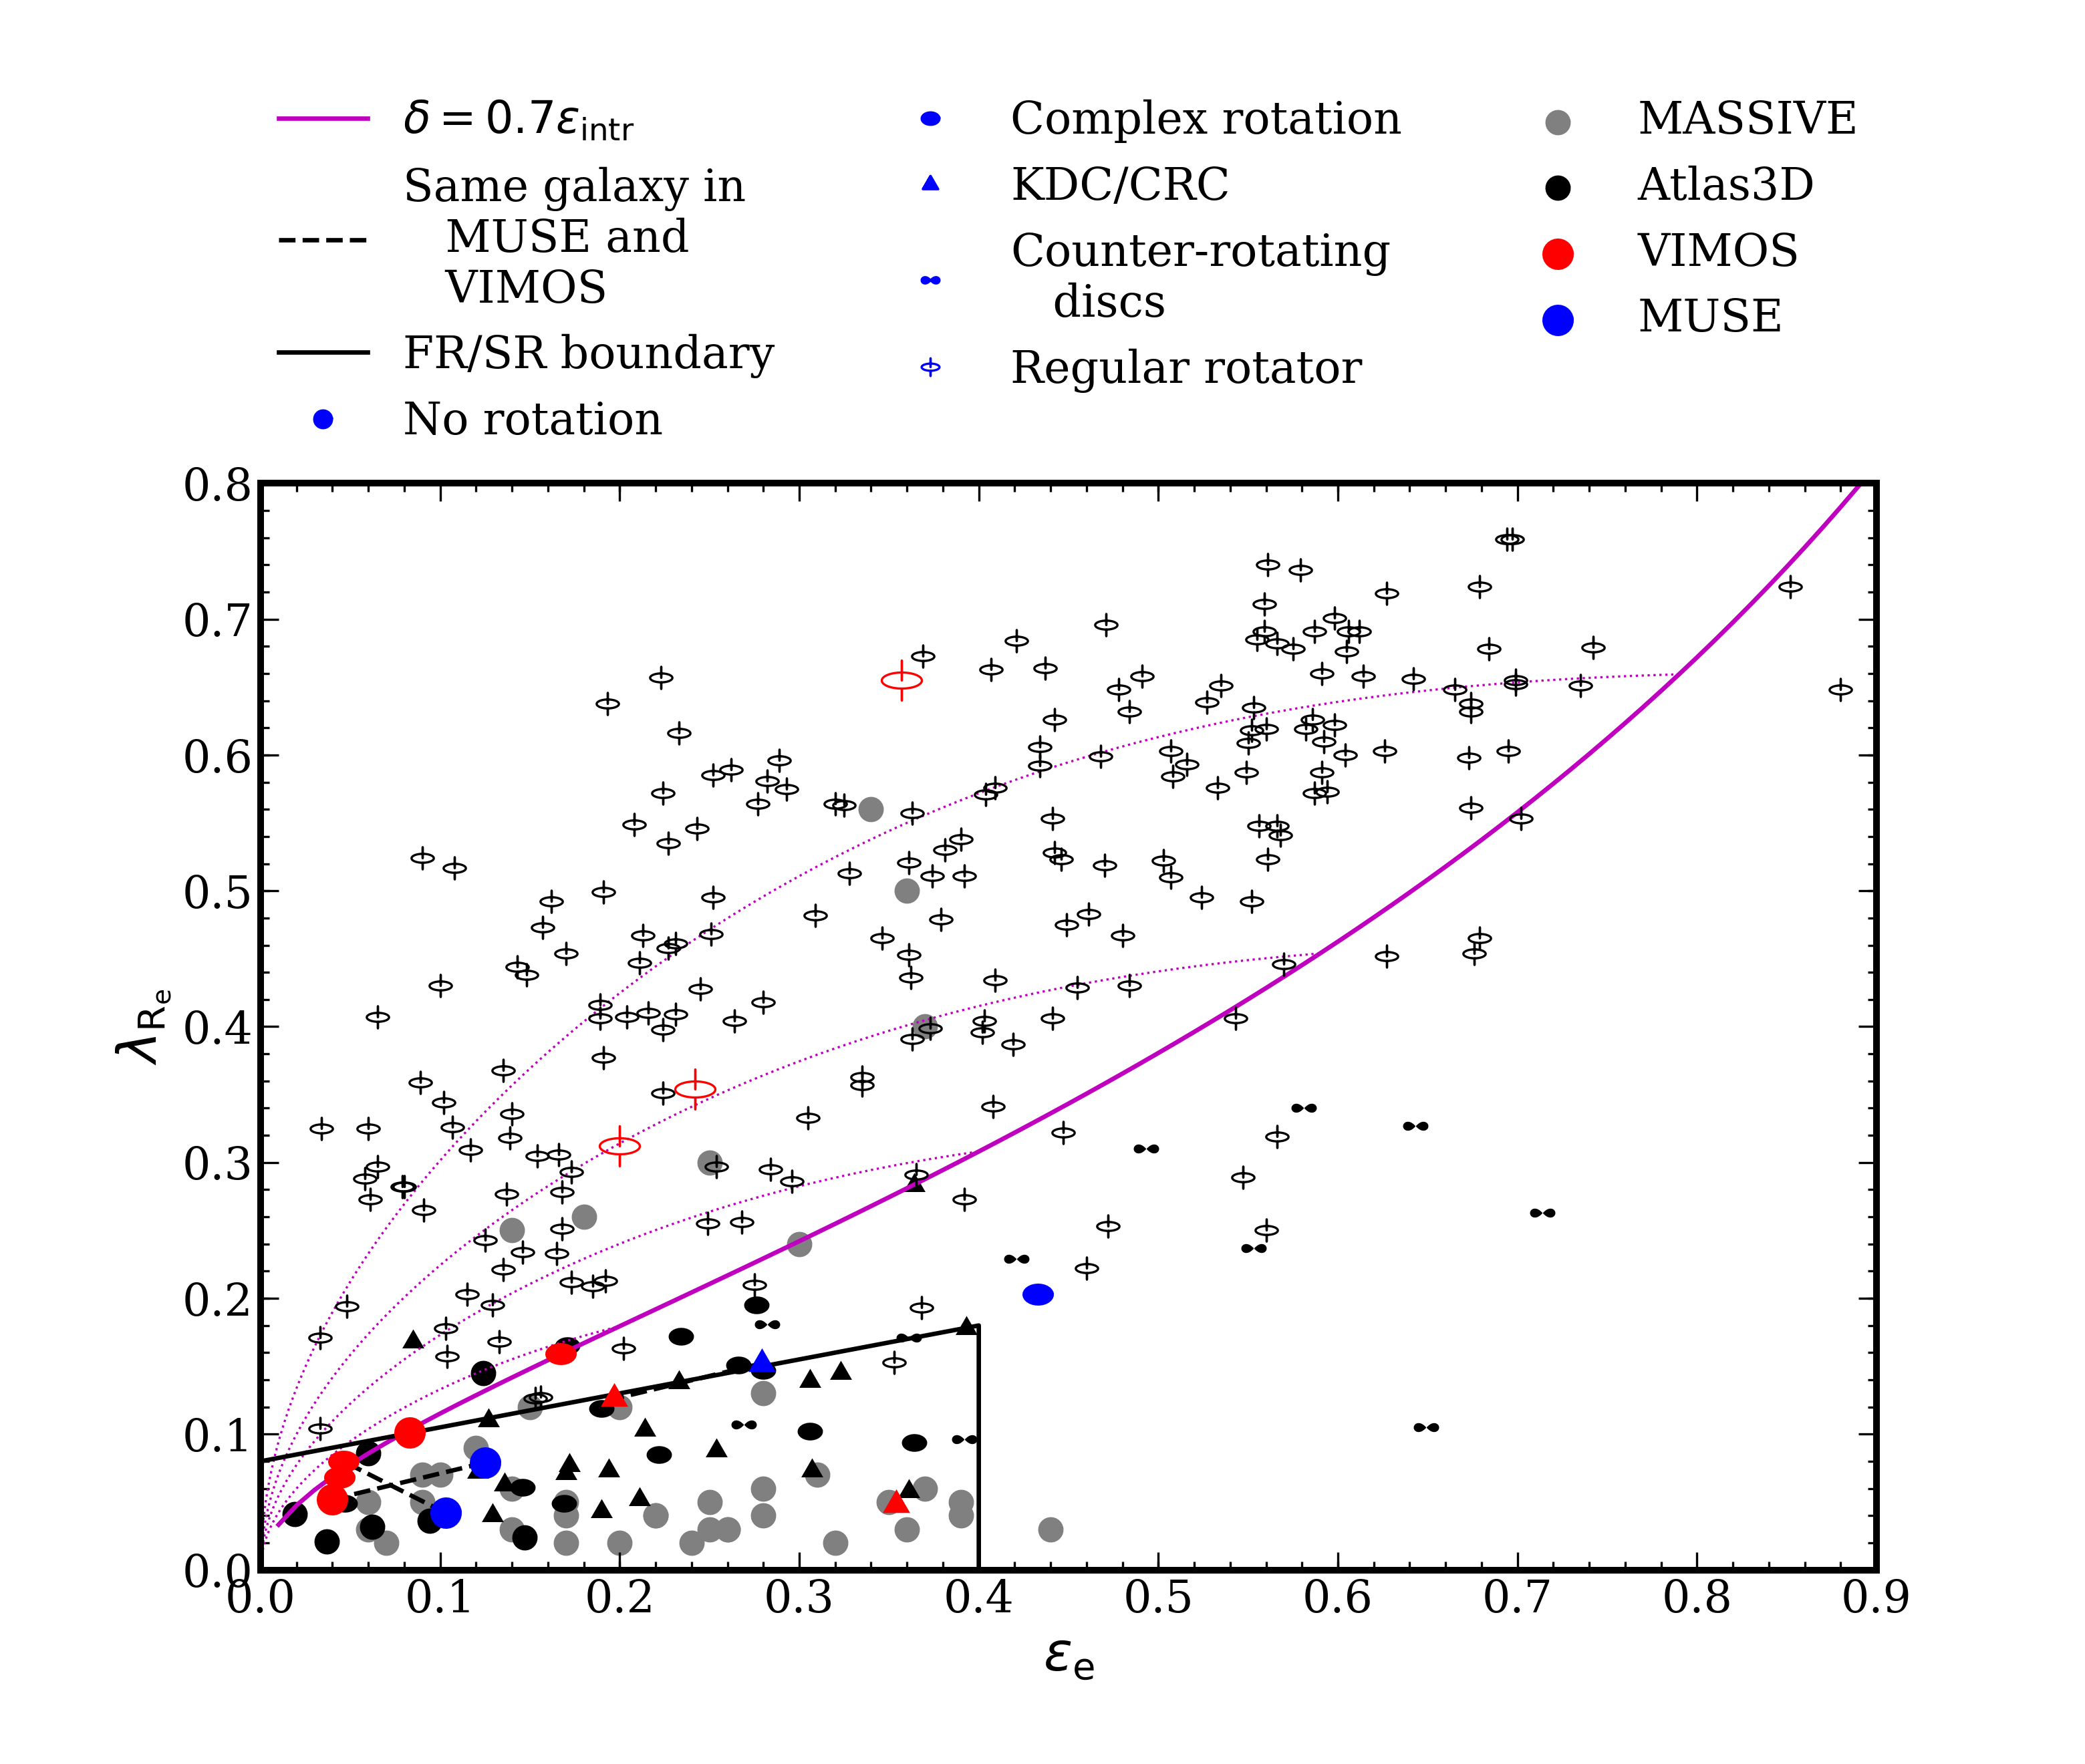
\includegraphics[width=\columnwidth]{lambda_R_ellipticity.png}
			\caption{$\lambda_\mathrm{R_e}$\,--\,ellipticity diagram. VIMOS and MUSE measurements are shown in red and blue, respectively. For comparison, Atlas$^\text{3D}$ galaxies \citep{Emsellem2011} are shown in black and MASSIVE galaxies \citep{Veale2017} in grey. The theoretical limit (edge-on systems) of disc-dominated galaxies is shown in solid magenta, with lines of constant intrinsic angular momentum but varying inclination in dotted magenta. The black solid lines show the limits of the fast-/slow-rotator classes. The MASSIVE survey does not report substructure, so the MASSIVE sample galaxies are shown with filled circles.}
			\label{fig:lambdaR_ellip}
		\end{figure}


		5 out of 11 galaxies, or $(45\pm13)$\%, are slow rotators. This is between that of the Atlas$^\text{3D}$ and MASSIVE projects, who find 13.1\% and 77.5\% of their sample galaxies to be slow rotators, respectively. As for the regular/non-regular rotators classification scheme, slow rotators are more likely to be found in higher mass galaxies and the three samples (Atlas$^\text{3D}$, MASSIVE and our Southern sample) have very different mass distributions (see upper panel of Fig.\,\ref{fig:SRmassFraction}).

		In order to account for the difference in mass distribution, we find the expected fraction of slow rotators in the Southern sample, $f'$, corrected to the mass distribution of the combined Atlas$^\text{3D}$ and MASSIVE samples (hereafter the A+M sample), as
		\begin{equation}
			f' = \sum_{i=0}^N N^\text{SS}_i f^\text{AM}_i \, , 
		\end{equation}
		where $N^\text{SS}_i$ is the number of Southern sample galaxies in the $i^\text{th}$ mass bin, $N^\text{AM}_i$ is the fraction of slow rotators in the $i^\text{th}$ mass bin in the A+M combined sample and $N$ is the total number of mass bins. In our case we use the $K$-band absolute magnitude ($M_K$) as a proxy for stellar mass, with bins of 0.5 mag. This gives an expected fraction of $f' = 0.64 \pm 0.06$, just consistent with our finding of $(45\pm13)$\% of the Southern sample galaxies being slow rotators. Again the large uncertainty reflects the low number statistics of the Southern sample. There is, therefore, no discernible difference in the fraction of galaxies that are slow-rotators between our radio-selected Southern sample and the optically-selected A+M sample, once differences in the mass distributions are taken into account. 

		\begin{figure}
			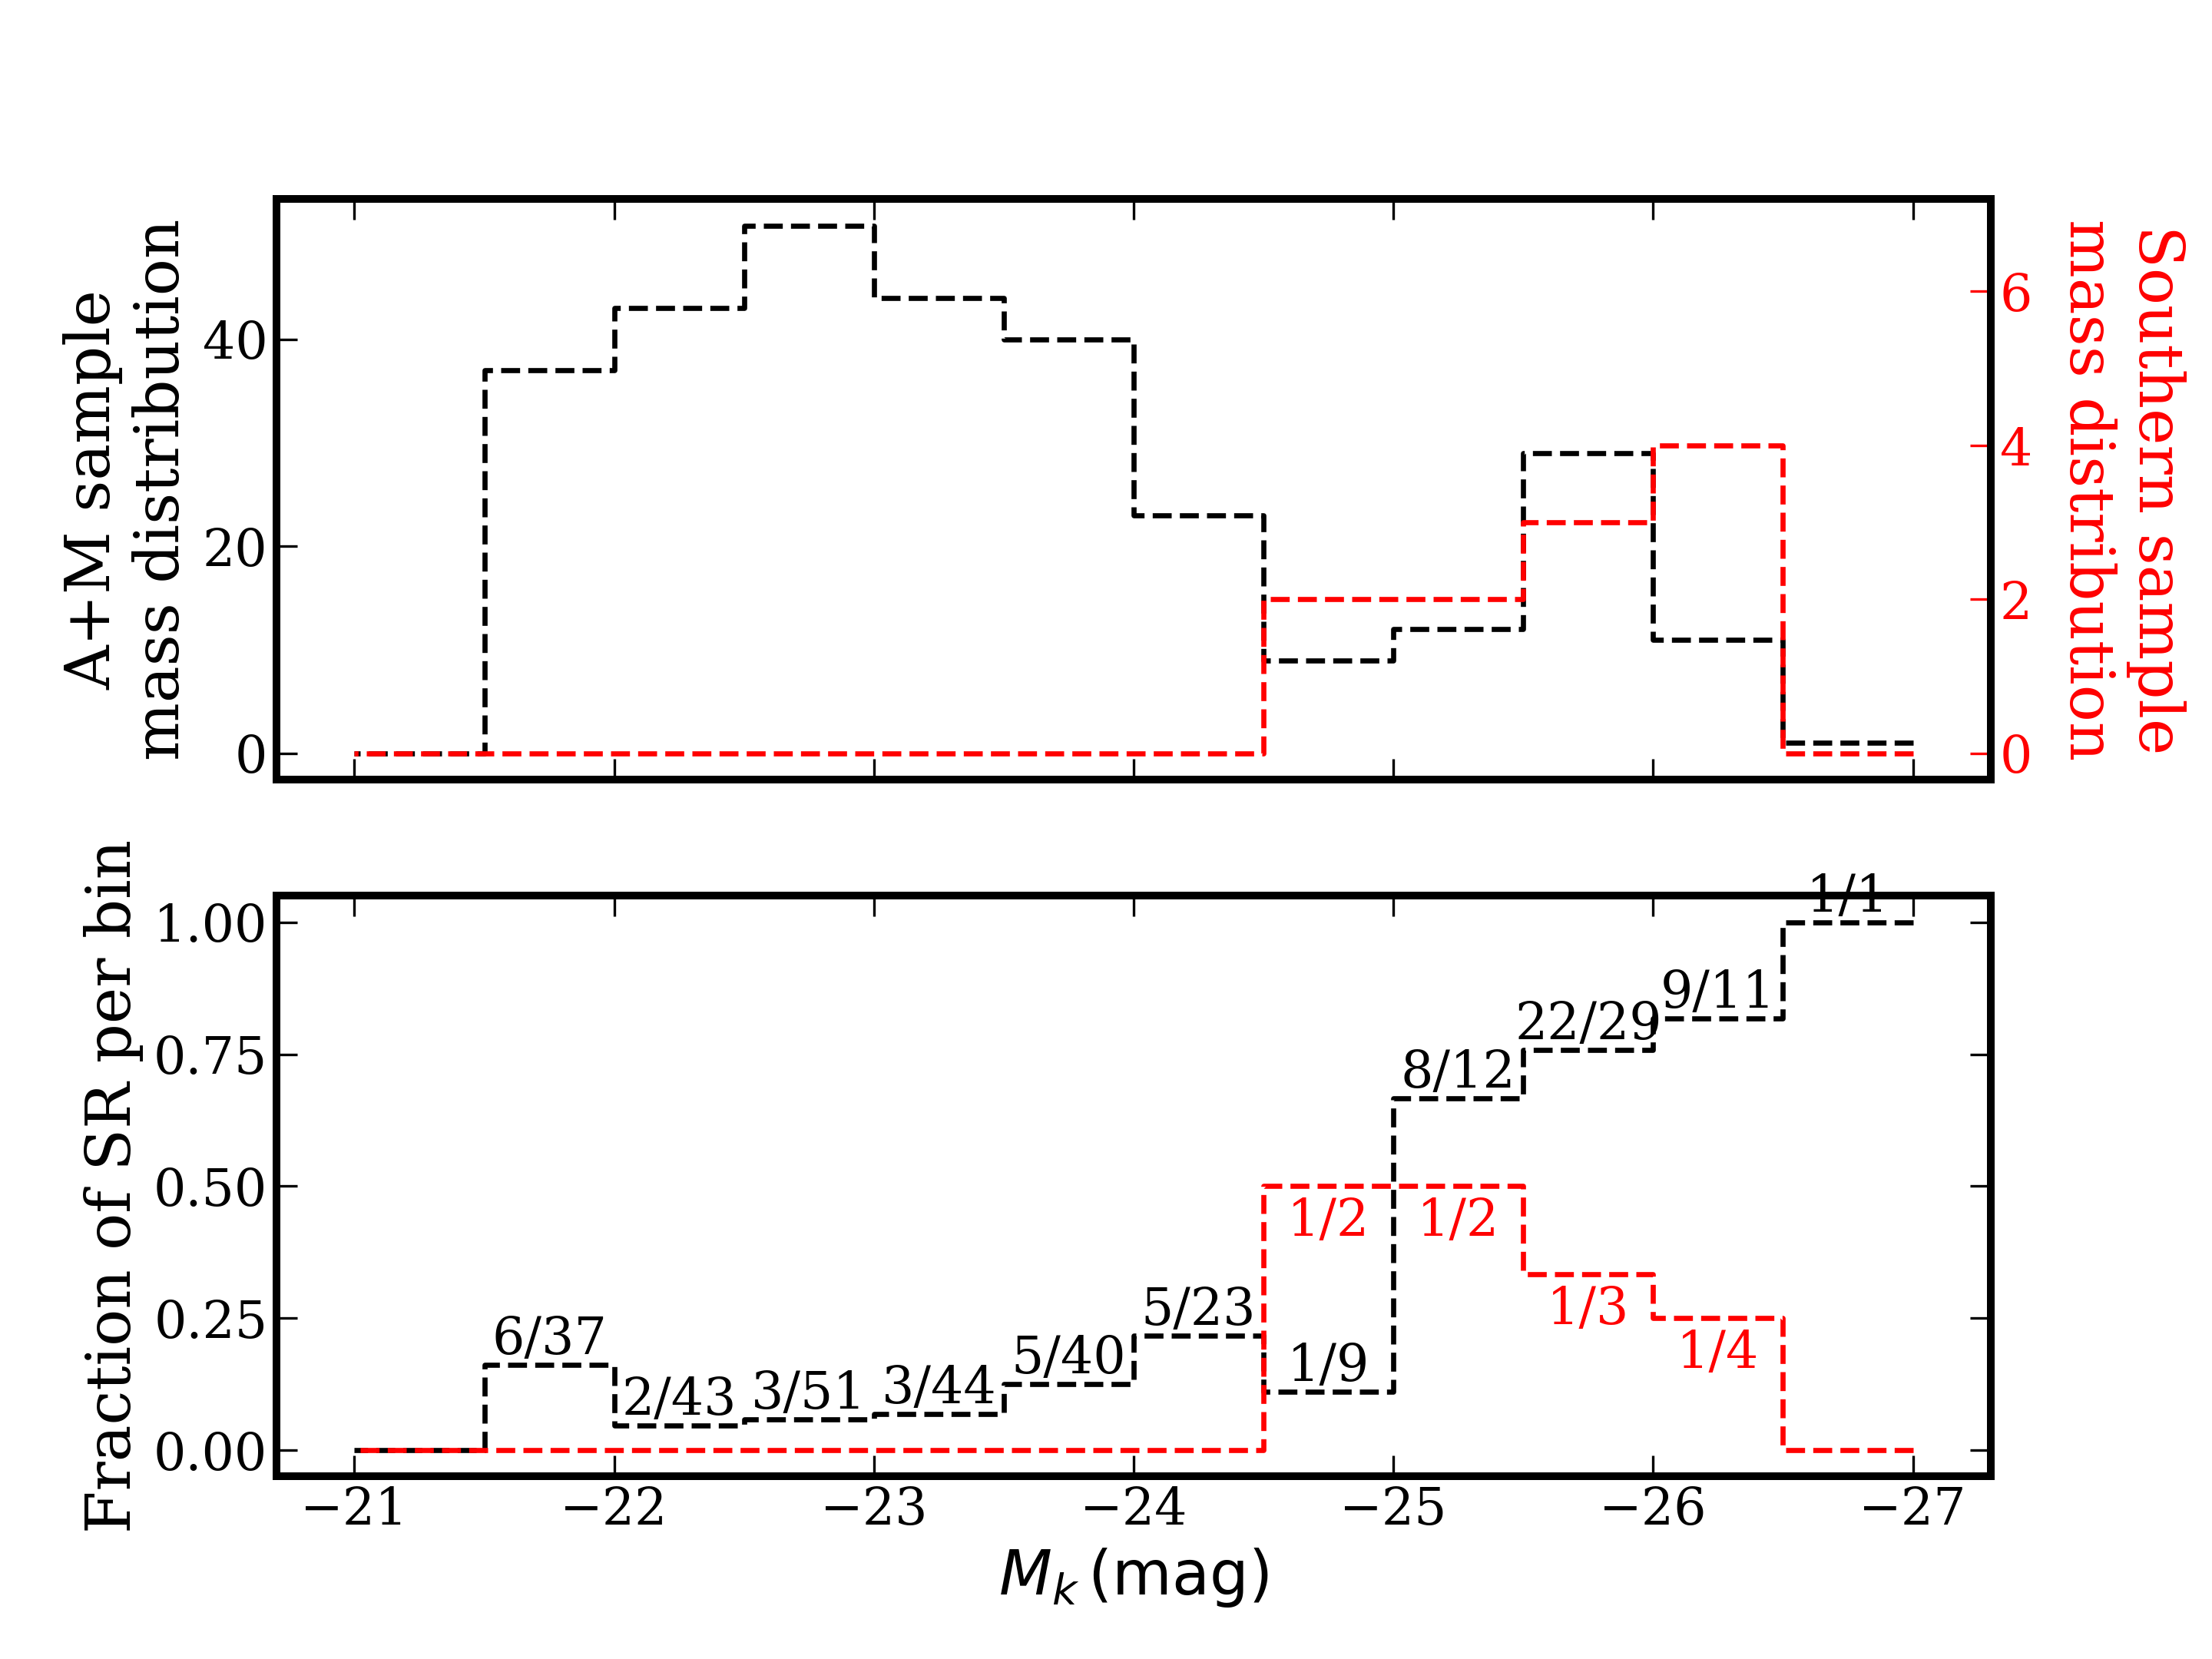
\includegraphics[width=\columnwidth]{M_k_binned.png}
			\caption{Upper panel: mass distribution of the A+M sample (black) and of our Southern sample (red). Lower panel: fraction of slow rotators within each mass bin. The labels list the number of slow rotators and total number of galaxies in each bin.}
			\label{fig:SRmassFraction}
		\end{figure}

	\subsection{Kinematic Features}
		In addition to this, we attempt to identify the kinematic features defined by \citet{Krajnovic2011} in an algorithmic way. However, the artefacts from the VIMOS quadrants confuse ellipse fitting algorithms so only maps derived from the MUSE data are classified in this way; kinematic features in maps derived from the VIMOS data are identified by eye. These classification are listed in Col.\,7 of Table \ref{tab:classify} and the corresponding kinematic group to which a given galaxy belongs to is given is Col.\,8. We observe 3 KDCs (although PKS 718-34 is only a tentative classification) such that $29\pm19$\% of non-regular rotators in our Southern sample definitely (not including PKS 718-34) contain KDCs (or $43\pm19$\% including PKS 718-34), with the large uncertainty reflecting the low-number statistics. This is consistent with the Atlas$^\text{3D}$ survey who found find $25\pm7$\% of non-regular rotators host KDCs \citep{Krajnovic2011}.


	\subsection{Intrinsic Shape}
		The misalignment angle between the photometric and kinematic position angle is given in Col.\,4 of Table \ref{tab:classify}. Misaligned systems may appear aligned in certain projections, but though aligned systems will be aligned in all projections, and a low value of $\Gamma_\text{kin}$ cannot be used to describe the intrinsic shape of an individual galaxy, but it can be interpreted within a statistical framework. However, a high value of $\Gamma_\text{kin}$ can give an insight into the intrinsic shape of an individual galaxy. We find all the regular rotators in our Southern sample, are consistent with having aligned photometry and kinematic position angles to within 11\degr, while non-regular rotators have a large range of values of $\Gamma_\text{kin}$. IC 1531, NGC7075 and PKS 718-34 all have very large uncertainties in the value of $PA_\text{phot}$ due to the VIMOS quadrant artefacts causing the fitting routine of \textsc{kinemetry} to become unreliable. 

		The lack of misalignments in regular rotators is consistent with \citet{Cappellari2007}, \citet{Krajnovic2011} and \citet{Fogarty2015}, who all showed that regular rotators almost always have aligned photometric and kinematic axes with very little scatter and that regular rotators with a significant misalignment are either interacting or strongly barred. The lack of misalignments suggests that the regular rotators (including those within our Southern sample) are consistent with being axisymmetric \citep{Cappellari2016}.

		Misalignments between the photometric and kinematic position angles are routinely observed for non-regular rotators. This generally implies a more triaxial intrinsic shape, although large misalignments are extremely rarely observed in galaxies with $\epsilon > 0.4$, suggesting that non-regular rotators are more spherical in shape \citep{Cappellari2016}. The non-regular rotators in our Southern sample indeed all have $\epsilon < 0.4$ showing that they are consistent with a fairly spherical, triaxial intrinsic shape.

\section{Absorption Line Strengths}
	\label{sec:absorption}
	Using the methods described in Section \ref{subsec:absorption} we produce maps of the absorption line strength indices for each galaxy (shown in Appendix \ref{sec:Maps}). Here we measure the Mg\,--\,velocity dispersion relation and compare our absorption line strength measurements to the literature. 

	\subsection{Mg\,--\,$\sigma$ relation}
		\label{subsec:Mgsigma}
		The Mg$_2$ absorption line index of \citet{Trager1998} has overlapping bandpasses with the Mg\,b index (also of \citeauthor{Trager1998}), but includes the MgH molecular absorption line, and is hence considered a molecular index and is measured in units of magnitude. \citet{Bender1993} observed the tight relationship between the global Mg$_2$ absorption line strength and logarithm of the central velocity dispersion, $\sigma_0$, in elliptical galaxies. They also noticed that residuals to the linear best-fitting appeared to be intrinsic as they have a near Gaussian shape about the median values, but do not seem to be correlated to any other galaxy property. 

		Since part of the red continuum band of the Mg$_2$ index is outside of the spectral range of VIMOS, we instead use the Mg\,b index. \citet{Ziegler1997} show there is an approximately linear relationship between Mg\,b and Mg$_2$, with a gradient of 14.3--15.5\,mag\,\AA$^{-1}$\ depending on metallicity. We thus use Mg\,b as a proxy for Mg$_2$. 

		Using an aperture with a radius of 2 arcsec on each datacube, we measure $\sigma_0$ and Mg\,b at a spectral resolution of 8.4\,\AA\ full-width half-maximum (FWHM), chosen such that the transformation functions of \citet{Vazdekis2010} can be used to change the literature measurements from the Lick/IDS system to the LIS. The results are shown in Fig.\,\ref{fig:globalMg} with the best-fitting linear relationship (found using \textsc{lts\_linefit} by \citealt{Cappellari2013}) shown by the solid black line. This has a gradient of $2.3 \pm 0.5 \,\mathrm{\AA\,dex^{-1}}$) and intrinsic scatter of $0.13 \pm 0.10 \, \mathrm{\AA}$. %Individual measurements for each galaxy are given in table \ref{tab:globalMg}.
		This is in very good agreement with the gradient found by \citet{Ziegler1997} for a sample of elliptical galaxies within Virgo and Coma using data from \citet{Dressler1987} of $2.5\,\mathrm{\AA\,dex^{-1}}$ (blue dotted line in Fig.\,\ref{fig:globalMg}), with an intrinsic scatter of 0.16\,\AA\ for galaxies with $\log \sigma_0 \geqslant 2.3$. 

		\begin{figure}
			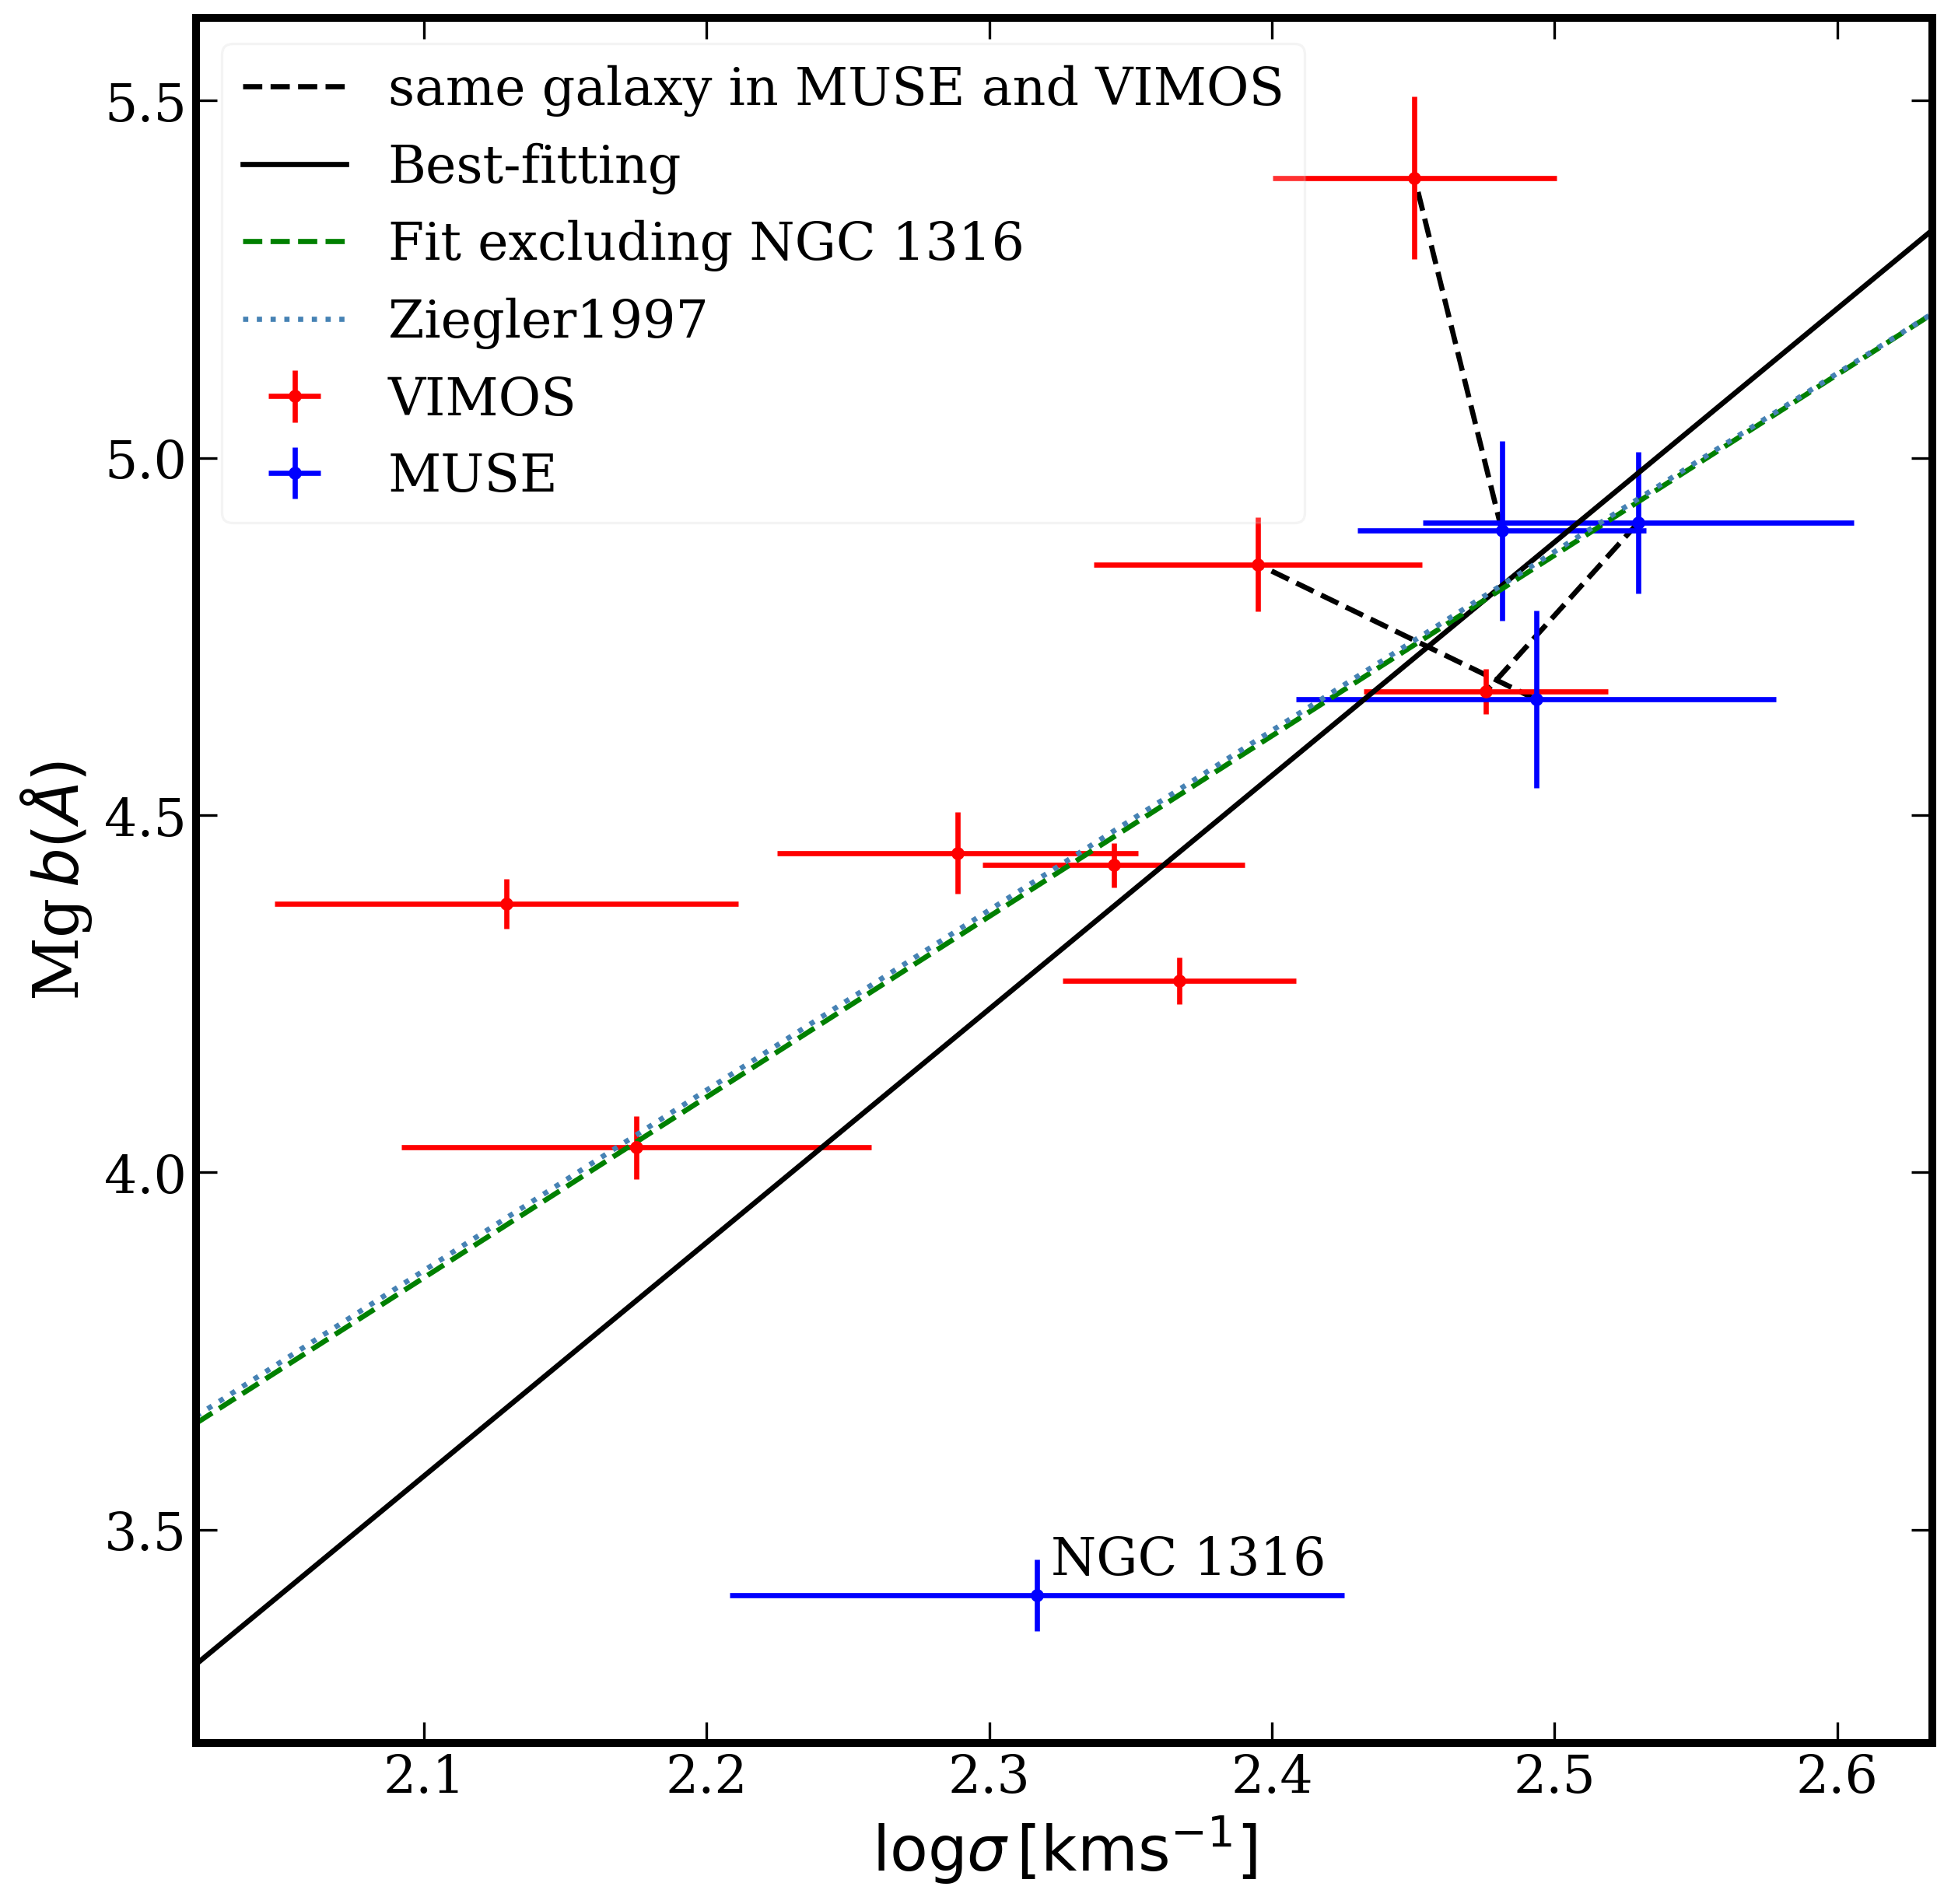
\includegraphics[width=\columnwidth]{Mg_sigma.png}
			\caption[Global Mg\,b\,--\,$\sigma$]{The Mg\,b\,--\,velocity dispersion relation using a 2\arcsec aperture. We find a similar gradient to our best-fitting (solid) as that found by \citet[; dotted line]{Ziegler1997}.}
			\label{fig:globalMg}
		\end{figure}

	\subsection{Comparison to the Literature}
		\label{subsec:Lit}
		Given that there is no well defined list of corrections (and methods) that is universally followed, care must be taken when making comparisons to the literature. When comparing to a particular paper we correct for the same effects described in the paper, but using our methods, as described in Section \ref{subsec:absorption}. As in Section \ref{subsec:Mgsigma} we use a resolution of 8.4\,\AA\ FWHM in order to use the transformation function provided by \citet{Vazdekis2010} from Lick/IDS system to the LIS.

		Table \ref{tab:litAbsorption} summarises our comparisons to the literature. For the comparison to \citet{Vazdekis2010}, we analysed the SAURON dataset\footnote{\url{http://www.strw.leidenuniv.nl/sauron/}} \citep{Emsellem2004} using the same analysis pipeline as for our Southern Sample. 


		\begin{table}
			\centering
		% \begin{threeparttable}
			\caption{Comparisons of measured absorption line indices to the literature. Comparisons to \citet{Rampazzo2005} are sampled at 7 radial apertures for each galaxy: 1.5, 2.5 and 10.0 arcsec and R$_e$/10, R$_e$/8, R$_e$/4 and R$_e$/2. Col.\,1: Index. Col.\,2: Number of galaxies in comparison. Col.\,3: Offset equals the mean of the measurements from the literature subtract our measurements. Col.\,4: Dispersion equals the standard deviation of the measurements from the literature subtract our measurements.}
			\label{tab:litAbsorption}
			% \begin{tabular*}{0.8\textwidth}{@{\extracolsep{\fill}}l r r r}
			\begin{tabular}{l r r r}
				\hline
				\hline
				Index 		& \multicolumn{1}{c}{N$_\mathrm{gals}$} & \multicolumn{1}{c}{Offset} & \multicolumn{1}{c}{Dispersion} \\
							& 		&\multicolumn{1}{c}{\AA}& \multicolumn{1}{c}{\AA} \\
				\hline
				\multicolumn{4}{c}{\citet{Vazdekis2010} (SAURON)} \\
				\hline
				H\,$\beta$ 	& 46		& -0.02\leavevmode\phantom{0}& 0.25\leavevmode\phantom{0}	\\
				Fe5015		& 46		& 0.66\leavevmode\phantom{0}& 0.34\leavevmode\phantom{0}	\\
				Mg\,b 		& 46		& 0.06\leavevmode\phantom{0}& 0.33\leavevmode\phantom{0}	\\
				\hline
				\multicolumn{4}{c}{\citet{Rampazzo2005} (VIMOS)} \\
				\hline
				G4300 		& 3 		& 2.29\leavevmode\phantom{0}& 0.11\leavevmode\phantom{0}	\\
				Fe4383 		& 3 		& 0.39\leavevmode\phantom{0}& 0.23\leavevmode\phantom{0}	\\
				Ca4455 		& 3 		& -0.19\leavevmode\phantom{0}& 0.09\leavevmode\phantom{0}	\\
				Fe4531 		& 3 		& 0.16\leavevmode\phantom{0}& 0.26\leavevmode\phantom{0}	\\
				H\,$\beta$ 	& 3 		& 0.17\leavevmode\phantom{0}& 0.12\leavevmode\phantom{0}	\\
				Fe5015 		& 3 		& -0.73\leavevmode\phantom{0}& 0.48\leavevmode\phantom{0}	\\
				Mg\,b 		& 3 		& -0.43\leavevmode\phantom{0}& 0.17\leavevmode\phantom{0}	\\
				\hline
				\multicolumn{4}{c}{\citet{Rampazzo2005} (MUSE)} \\
				\hline
				H\,$\beta$ 	& 2 		& -0.28\leavevmode\phantom{0}& 0.17\leavevmode\phantom{0}	\\ 
				Fe5015 		& 2 		& 0.87\leavevmode\phantom{0}& 0.34\leavevmode\phantom{0}	\\ 
				Mg\,b 		& 2 		& 0.31\leavevmode\phantom{0}& 0.14\leavevmode\phantom{0}	\\
				Fe5270 		& 2 		& -0.11\leavevmode\phantom{0}& 0.15\leavevmode\phantom{0}	\\
				Fe5335 		& 2 		& 0.08\leavevmode\phantom{0}& 0.15\leavevmode\phantom{0}	\\
				Fe5406 		& 2 		& 0.16\leavevmode\phantom{0}& 0.07\leavevmode\phantom{0}	\\
				Fe5709 		& 2 		& 0.11\leavevmode\phantom{0}& 0.10\leavevmode\phantom{0}	\\
				Fe5782 		& 2 		& -0.03\leavevmode\phantom{0}& 0.11\leavevmode\phantom{0}	\\
				NaD 		& 2 		& 0.90\leavevmode\phantom{0}& 0.41\leavevmode\phantom{0}	\\
				TiO1 (mag)	& 2 		& -0.004	& 0.003	\\
				TiO2 (mag)	& 2 		& -0.011	& 0.007	\\
				\hline
				\multicolumn{4}{c}{\citet{Ogando2008} (VIMOS)} \\
				\hline
				H\,$\beta$ 	& 6 		& 0.07\leavevmode\phantom{0}& 0.60\leavevmode\phantom{0}	\\
				Fe5015 		& 6 		& -0.09\leavevmode\phantom{0}& 0.15\leavevmode\phantom{0}	\\
				Mg\,b 		& 6 		& -0.70\leavevmode\phantom{0}& 0.08\leavevmode\phantom{0}	\\
				\hline
				\multicolumn{4}{c}{\citet{Ogando2008} (MUSE)} \\
				\hline
				H\,$\beta$ 	& 3 		& -0.04\leavevmode\phantom{0}& 0.23\leavevmode\phantom{0}	\\ 
				Fe5015 		& 3 		& -0.16\leavevmode\phantom{0}& 0.33\leavevmode\phantom{0}	\\ 
				Mg\,b 		& 3 		& -1.10\leavevmode\phantom{0}& 0.26\leavevmode\phantom{0}	\\
				Fe5270 		& 3 		& -0.66\leavevmode\phantom{0}& 0.16\leavevmode\phantom{0}	\\
				Fe5335 		& 3 		& -0.66\leavevmode\phantom{0}& 0.11\leavevmode\phantom{0}	\\
				Fe5406 		& 3 		& -0.51\leavevmode\phantom{0}& 0.06\leavevmode\phantom{0}	\\
				Fe5709 		& 3 		& -0.22\leavevmode\phantom{0}& 0.08\leavevmode\phantom{0}	\\
				NaD 		& 3 		& -1.57\leavevmode\phantom{0}& 0.16\leavevmode\phantom{0}	\\
				\hline
				\hline
			\end{tabular}
		% 	\begin{tablenotes}
		% 	\footnotesize
		% 	\note Comparisons to \citet{Rampazzo2005} are sampled at 7 radial apertures for each galaxy: 1.5, 2.5 and 10.0 arcsec and R$_e$/10, R$_e$/8, R$_e$/4 and R$_e$/2. 
		% 	\item Col.\,1: Index. Col.\,2: Number of galaxies in comparison. Col.\,3: Offset equals the mean of the measurements from the literature subtract our measurements. Col.\,4: Dispersion equals the standard deviation of the measurements from the literature subtract our measurements.
		% 	\end{tablenotes}
		% \end{threeparttable}
		\end{table}

		We find a very large offset for the G4300 index with respect to the results of \citet{Rampazzo2005}. As noted above, this index is extremely sensitive to the stellar velocity dispersion correction and we measure an average difference in the stellar velocity dispersion to that measured by \citet{Rampazzo2005} of $21\,\mathrm{km\,s^{-1}}$. This may be enough to account for the difference in the measurements.

		We also observe that the offset in the Fe5015 index is also quite large in comparisons with \citet{Rampazzo2005} and \citet{Vazdekis2010}. In the case of the comparison with \citet{Rampazzo2005} we suggest that the difference is due to differences in method for accounting for the [\ion{O}{iii}] emission lines, however the origin of the offset is less clear in case of the comparison with \citet{Vazdekis2010}. 

		Other than G4300 and Fe5015, the comparisons show fairly consistent agreement with literature measurements although the dispersion of the comparisons are fairly large. We suggest that the translation between Lick and LIS systems may be the source of this spread.

\section{Stellar Populations}
	\label{sec:stellarPop}
	We have assumed that a given spectrum from our Southern sample can be well approximated by a SSP. We use the method described in Section \ref{subsubsec:stellarPop} to produce maps of the most-likely SSP characteristics: age ($t$), metallicity ($Z/H$) and alpha-element enhancement ($\alpha$/Fe) from the absorption line strength maps (see Appendix \ref{sec:Maps}).

	In general, our sample galaxies show old, metal rich and alpha enhanced SSPs; qualities which ETGs are well known for. The exceptions are NGC 612 and NGC 1316. NGC 1316 shows a very young stellar population (our fit of $t \approx 2$\,Gyr agrees with that of \citealt{Kuntschner2000}, but is conflicting with the older and less metal rich stellar population of \citealt{Koleva2011} who found $t=4.5 \pm 0.3 \,\mathrm{Gyr}$ and $\mathrm{[Fe/H]}=0.12 \pm 0.01 \,\mathrm{dex}$ for an aperture covering the central 0.1 kpc). NGC 3557 is notable for containing a significantly younger ($t\approx 4$\,Gyr) core of about 10\arcsec\ diameter and NGC 3100 has a branch of young stars ($\approx 4$\,Gyr) along the southeast branch of the molecular gas (cyan contours).

	\subsection{Radial Gradients in Stellar Populations}
		\label{subsec:popGrad}

		\citet{Koleva2011} showed that while individual galaxies can have a wide range of radial gradients of age and metallicity, the mean gradient (within a mass bin) is uniform across a large mass range. They assume a linear relationship between $\log t$ or [Fe/H] and $\log (R/\mathrm{R_e})$. We repeat this fit with our Southern Sample with the results shown in Table \ref{tab:popGrad}. 

		\begin{table}
			\centering
			\caption{The radial gradients of the most-likely SSP models.}
			\label{tab:popGrad}
			\begin{tabular}{l c c}
				\hline
				\hline 
				Galaxy 	& $\Delta_\text{log age}$ & $\Delta_\text{[Fe/H]}$ \\ 
					& dex\,arcsec$^{-1}$ & dex\,arcsec$^{-1}$ \\
				\hline
				ESO 443-G024 & $0.019 \pm 0.013$ & $-0.01 \pm 0.02$ \\
				IC 1459 	& $0.003 \pm 0.002$ & $0.00 \pm 0.06$ \\
				IC 1531 	& $0.012 \pm 0.015$ & $0.01 \pm 0.02$ \\
				IC 4296		& $0.000 \pm 0.002$ & $0.04 \pm 0.08$ \\
				NGC 612 	& $0.068 \pm 0.060$ & $-0.11 \pm 0.02$ \\
				NGC 1316 	& $0.001 \pm 0.002$ & $0.05 \pm 0.03$ \\
				NGC 1399 	& $0.001 \pm 0.002$ & $0.10 \pm 0.09$ \\
				NGC 3100 	& $0.000 \pm 0.010$ & $-0.06 \pm 0.01$ \\
				NGC 3557 	& $0.048 \pm 0.039$ & $-0.05 \pm 0.05$ \\
				NGC 7075 	& $0.007 \pm 0.011$ & $-0.07 \pm 0.02$ \\
				PKS 718-34  & $0.002 \pm 0.009$ & $-0.17 \pm 0.03$ \\
				\hline
				\hline
			\end{tabular}
		\end{table}

		We find average gradients of $\Delta_\text{log age} = 0.014\pm0.007 \,\mathrm{dex \, arcsec^{-1}}$ and $\Delta_\text{[Fe/H]} = -0.03\pm0.01 \, \mathrm{dex \, arcsec^{-1}}$. This is consistent with \citet{Koleva2011} who, for elliptical galaxies found average gradients of $0.06\pm0.09 \, \mathrm{dex \, arcsec^{-1}}$ and $-0.26\pm0.08 \, \mathrm{dex \, arcsec^{-1}}$ for the age and metallicity gradients, respectively. For S0s they find flatter corresponding gradients of $0.01\pm0.11\, \mathrm{dex \, arcsec^{-1}}$ and $-0.12\pm0.13\, \mathrm{dex \, arcsec^{-1}}$. 

	\subsection{Kinematically-Decoupled Cores}
		\label{subsec:popKDC}
		\citet{Kuntschner2010} found that kinematically-decoupled cores (KDCs) exist in two classes: they are either small or contain an old stellar population. The size of the KDC is defined as the radius of the region surrounding the KDC where the superposition of the two components (the KDC and the host galaxy) results in a local minimum in the mean velocity. The age of the most-likely SSP model for the spatially integrated spectrum within an aperture 1\arcsec\ on the centre of the galaxy is taken as the KDC's age.

		The small KDCs are too small to be spatially resolved by our data, and thus are not considered here. The large KDCs are typically embedded in slow rotators. They have no limit on the age of their stellar populations suggesting that the stars within the KDC dominate in total mass as well as surface brightness. Thus, they do not fade into their host galaxies as they age unlike the small KDCs \citep{Kuntschner2010}. \citet{Bois2011} showed major mergers may well result in such large KDCs if the initial spin axis of the progenitor galaxy with the lowest bulge-to-disc ratio (later-type) is anti-parallel to the orbital angular momentum vector. 

		In Fig.\,\ref{fig:KDC} we show the age and size of the 3 KDCs hosted by galaxies in our Southern sample. We include PKS 718-34 here but stress it is only tentatively classified as containing a KDC. As can be seen from Fig.\,\ref{fig:KDC}, PKS 718-34 would be an extremely large KDC, but is still is consistent with the findings of \citet{Kuntschner2010}.

		\begin{figure}
			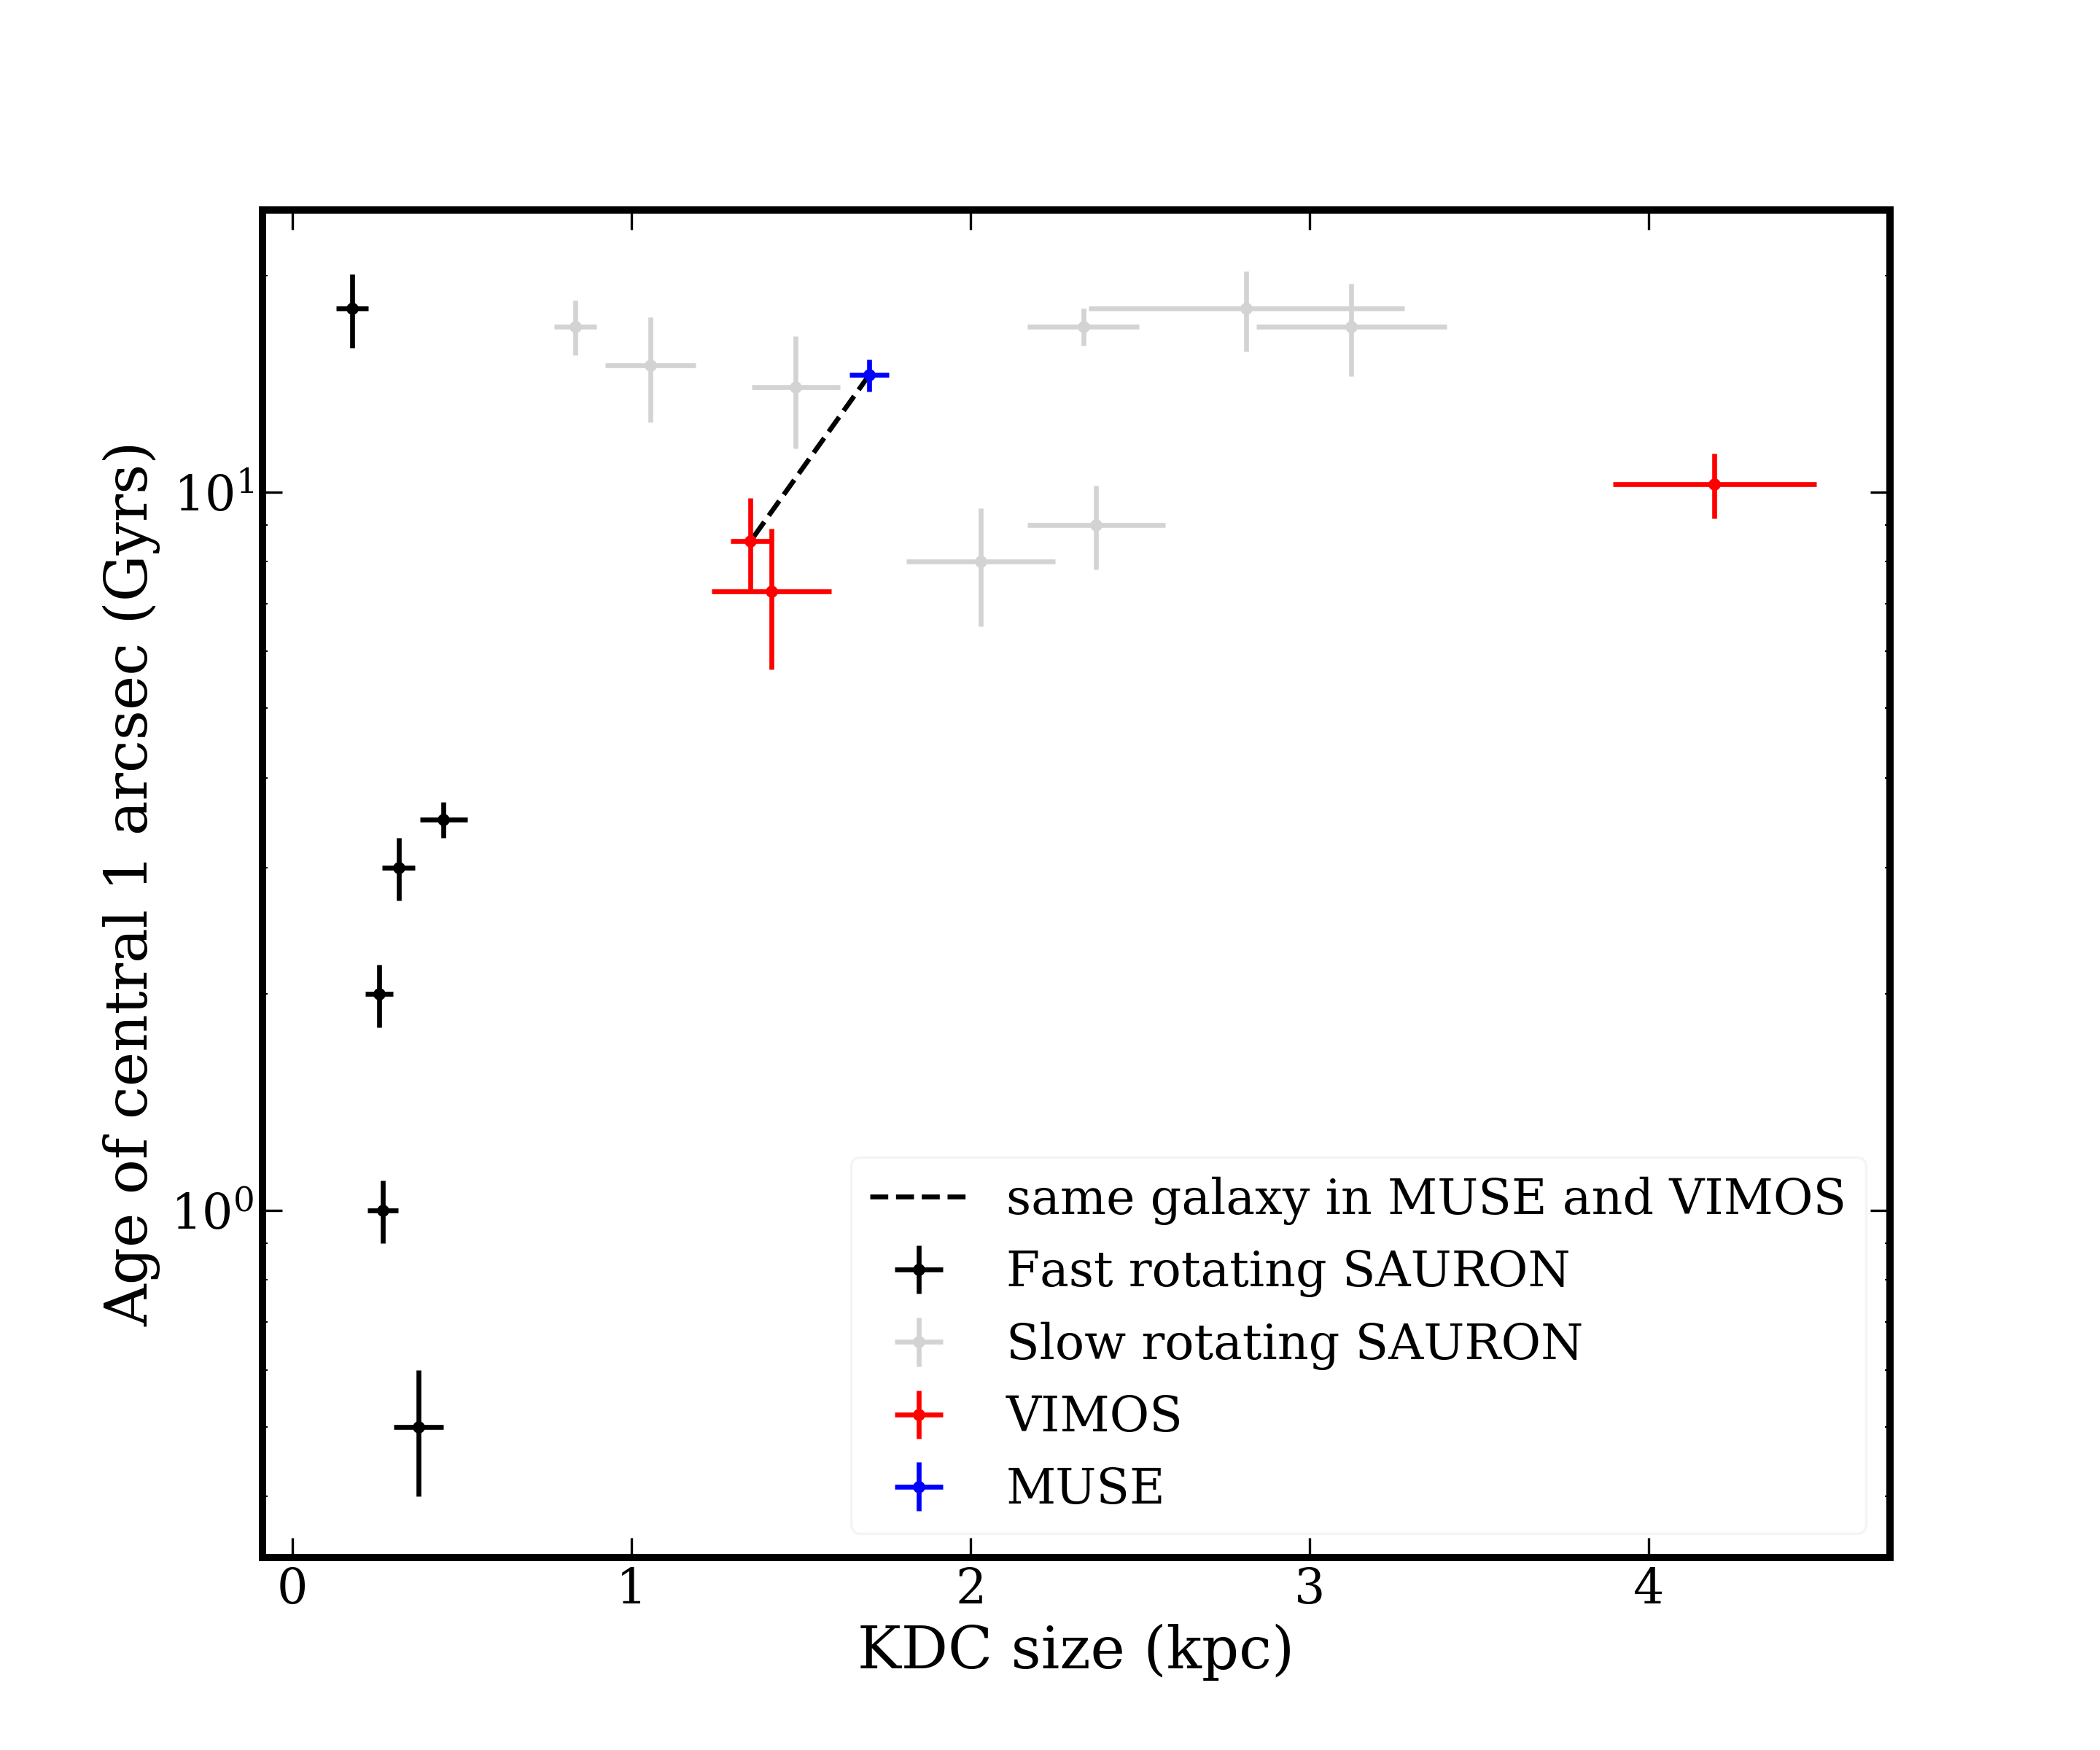
\includegraphics[width=\columnwidth]{KDC_size_age.png}
			\caption[KDC dichotomy]{The KDC size\,--\,age relation. KDCs exist in two classes: old or small. VIMOS is in red, MUSE in blue and SAURON from \citet{Kuntschner2010} in black and gray for fast and slow rotators respectively.}
			\label{fig:KDC}
		\end{figure}


\section{Ionized Gas Distribution, Kinematics and Ionization}
	\label{sec:gas}
	Using the methods described in Section \ref{subsubsec:EmissionFit}, we find the best-fitting line-of-sight velocity distribution (LOSVD; assumed to be Gaussian and parametrised by the mean velocity and velocity dispersion only) of the emission lines in each bin. Images of the Southern Sample galaxies in the [\ion{O}{iii}]$\lambda\lambda$4957,5007 lines are shown in Appendix \ref{sec:Maps} (we choose to show [\ion{O}{iii}] as detections of all emission lines require a detection of [\ion{O}{iii}] first, see Section \ref{subsubsec:EmissionFit}). Only 4 galaxies of the Southern Sample have emission lines detected outside of their central region (IC 1459, NGC 612, NGC 1316 and NGC 3100). Of the remaining 7 galaxies, NGC 1399 and PKS 718-34 have no detection of H$\beta$ in their spatially-resolved map (although we do detect H$\beta$ in the spatially-integrated spectrum of NGC 1399; see below), while the other 5 galaxies are only detected in their centre. All other emission lines have similar distributions, but with different fluxes.

	As can be seen from the maps in Appendix \ref{sec:Maps}, both NGC 612 and NGC 3100 have significant off-centre clouds of ionized gas. The latter is spatial coincident with both the radio jet and the gap in the CO ring, while former seems to no link with either the radio jet (a massive scale jet extending several $\sim 200$\,kpc to the east and west of the galaxy centre) or the CO. 


	\begin{table*}
		\centering
	% \begin{threeparttable}
		\caption{Gas masses of the Southern Sample galaxies. Col.\,1: Galaxy. Col.\,2: \ion{H}{ii} mass derived from the H$\beta$ line in the VIMOS data, assuming a Balmer decrement of 2.85. Col.\,3: \ion{H}{ii} mass derived from the H$\alpha$ line in the MUSE data. Col.\,4: Balmer decrement measured from the MUSE data. Col.\,5: Main source of ionizing radiation (see Section \ref{subsec:Diagnostics} for a description of the different classes). -- means we have no data.}
		\label{tab:gasMass}
		% \begin{tabular*}{\textwidth}{@{\extracolsep{\fill}}l r r r l}
		\begin{tabular}{l c c c c}
			\hline
			\hline
			Galaxy & \multicolumn{2}{c}{\ion{H}{ii} Mass} & Balmer & LINER/ \\
			& VIMOS\tnote{a} & MUSE & Decrement & Seyfert \\
			& ($\log\mathrm{M_\odot}$) & ($\log\mathrm{M_\odot}$) & \\
			\hline
			ESO 443-G024 & $5.02 \pm 0.01$ 	& --  		& -- & LINER \\
			IC 1459 	& $5.21 \pm 0.01$	& $5.50 \pm 0.01$ & $4.54 \pm 0.12$ & LINER-AGN\\
			IC 1531 	& $5.09 \pm 0.01$	& -- 		& -- & Seyfert 2\\
			IC 4296		& $5.43 \pm 0.01$	& $< 4.48$ 	& \tnote{b} & LINER-AGN \\
			NGC 612 	& $6.00 \pm 0.01$ 	& -- 		& -- & LINER-AGN \\
			NGC 1316 	& -- 				& $ 5.29 \pm 0.01$ & $3.52 \pm 0.11$ & LINER-AGN \\
			NGC 1399 	& $< 3.86$ 			& $ 4.54 \pm 0.01$ & $< 21.4$\tnote{c} & LINER \\
			NGC 3100 	& $5.26 \pm 0.01$	& -- 		& -- & LINER-AGN \\
			NGC 3557 	& $4.61 \pm 0.02$ 	& -- 		& -- & LINER \\
			NGC 7075 	& $4.68 \pm 0.01$	& -- 		& -- & LINER \\
			PKS 718-34  & $< 5.08$	 		& -- 		& -- & Passive \\
			\hline
			\hline
			\multicolumn{5}{L{.7\linewidth}}{$^{a}$The VIMOS flux calibration and thus the derived gas masses are only approximate (see Section \ref{sec:obs} for more detail on the flux calibration).} \\
			\multicolumn{5}{L{.7\linewidth}}{$^{b}$Both H$\alpha$ and H$\beta$ are not detected with A/N $>2.5$, so no information can be gained.} \\
			\multicolumn{5}{L{.7\linewidth}}{$^{c}$H$\beta$ is not detected with A/N $> 2.5$, so the fit is unreliable (hence an upper limit).}
		\end{tabular}
	% 	\begin{tablenotes}
	% 	\footnotesize
	% 	\note Col.\,1: Galaxy. Col.\,2: \ion{H}{ii} mass derived from the H$\beta$ line in the VIMOS data, assuming a Balmer decrement of 2.85. Col.\,3: \ion{H}{ii} mass derived from the H$\alpha$ line in the MUSE data. Col.\,4: Balmer decrement measured from the MUSE data. Col.\,5: Main source of ionizing radiation (see Section \ref{subsec:Diagnostics} for a description of the different classes). -- means we have no data.
	% 	\item [a] The VIMOS flux calibration and thus the derived gas masses are only approximate (see Section \ref{subsec:VIMOSreduction} for more detail on the flux calibration).
	% 	\item [b] Both H$\alpha$ and H$\beta$ are not detected with A/N $>2.5$, so no information can be gained.
	% 	\item [c] H$\beta$ is not detected with A/N $> 2.5$, so the fit is unreliable (hence an upper limit). 
	% 	\end{tablenotes}
	% \end{threeparttable}
	\end{table*}




	Total ionized gas masses are derived using the prescription of \citet{Sarzi2005}. This is a very rough calculation and the values should not be used for quantitative applications. The approach follows \citet{Kim1989}, whereby
	\begin{equation}
		\left(\frac{M_\text{\ion{H}{ii}}}{M_\odot}\right) = 280 \left(\frac{D}{10\, \mathrm{Mpc}}\right)^2 \left(\frac{F(\mathrm{H\alpha})}{10^{-14} \, \mathrm{erg \, s^{-1} \, cm^{-2}}}\right) \left(\frac{10^3 \, \mathrm{cm^{-3}}}{n_\mathrm{e}}\right) \, ,
	\end{equation}
	where $M_\text{\ion{H}{ii}}$ is the total mass of \ion{H}{ii} in the galaxy, $D$ is the galaxy distance, and $F(\mathrm{H\alpha})$ is the H$\alpha$ flux measured from the spectrum created by summing spatially all spaxels within an aperture of $\frac{R_\mathrm{e}}{2}$ (chosen to exclude outer noisy regions of the observations, but include spatially extended gas regions). This method assumes an electron density $n_\mathrm{e} = 100 \, \mathrm{cm^{-3}}$, a temperature of $10^4$ K and case-B recombination (electrons above 13.6\,eV are not reabsorbed; e.g.\ \citealt[p.\,74]{Osterbrock1974}). Like \citet{Sarzi2005}, we only claim a detection if the amplitude-to-noise ratio (A/N) is $>4$ for [\ion{O}{iii}] and $>2.5$ for H$\beta$ or H$\alpha$. Upper limits are calculated using the $1\sigma$ noise level (see Section \ref{subsubsec:EmissionFit}).

	Our calculated gas masses are given Table \ref{tab:gasMass} and are at the upper limit of, and possibly exceed, the typical masses observed in ETGs. Given that our sample contains particularly massive galaxies, high ionized gas masses are not unexpected, however.

	\subsection{Ionized Gas Kinematics}
		\label{subsec:GasKin}
		Map of the best-fitting kinematics (mean velocity and velocity dispersion), as found with the methods described in Section \ref{subsubsec:EmissionFit} for the 4 galaxies (IC 1459, NGC 612, NGC 1316 and NGC 3100) with detected spatially-extended emission lines are shown in Appendix \ref{sec:Maps}. Due to that fact that, unlike stars, gas is dissipational, it is to be expected that given sufficient time, the ISM will always settle into a disc. These maps show that the ISM of the Southern sample galaxies varies from largely settled discs in IC 1459 and NGC 612 to more disordered kinematics of NGC 3100 and a possible inflow in NGC 1316.

		It is immediately clear when comparing the mean stellar velocity maps to the mean gas velocity maps that where gas is detected, its angular momentum is not often aligned with that of the stars. A misalignment between the kinematics of the stars and gas suggests an external origin for the gas (e.g.\ accretion or wet merger). However it should be noted that the converses is not necessarily true: aligned kinematics is consistent with an internal origin (e.g.\ stellar-mass loss), but it does \emph{not} require it \citep[e.g.][]{Davis2011a}. 

		We now comment on each galaxy in turn.

		\paragraph{IC 1459} has ionized gas counter-rotating with respect to the stellar kinematically-decoupled core, and also rotating independently from the rest of the galaxy. \citet{Franx1988} claim that the rotation of the gas is aligned with that of the stars outside of the KDC, however we observe outer stellar kinematics to be non-rotating. As the stellar disc did not survive the merger even that created the KDC, it is unlikely that the gas in IC 1459 progenitor galaxy survived. The lost gas may, however, have been re-accreted. Alternatively, the ISM may have yet another external origin. 

		\paragraph{NGC 612} has well aligned stellar and gaseous kinematics. The misalignment between the position angle of the stellar and gas kinematics (using the method described in Section \ref{subsubsec:KinPA}) is just $1\fdg0\pm0\fdg7$, consistent with an internal origin for the gas. This adds to the evidence that NGC 612 has not undergone a major merger (major mergers exhaust galaxies of their gas and destroy a stellar disc) and suggests that, the fueling and powering of the radio jet must be a purely secular process. 


		\paragraph{NGC 1316} is a complex object. Since there are redshifted emission lines with respect to the rest frame of the galaxy on both sides of the galaxy, the gas is not in a settled disc and that there must be some inflow/outflows. 
		% We used a fitting routine based on the method of \citet{Swinbank2012}, \citet{Stott2016} and Tiley et.al.\ (in prep.) to fit an exponential disc (middle panel of Fig.\ \ref{fig:Inflow}) to the ionized gas mean velocity map (left panel), with the residuals shown in the right panel of Fig.\ \ref{fig:Inflow}. This shows a large residual on the southwest side of the galaxy, which we interpret as an inflow towards the nucleus, almost perpendicular to the radio jet. However, there are still significant residuals in other parts of the galaxy, suggesting that the model may not be a good representation of the reality of the galaxy, thus other interpretations are possible, and better quality data (longer exposure times) are required to add certainty to this interpretation. Nevertheless, it is clear that the gas in not in a settled disc. 
		Without filling in some of the regions were we do not detect emission lines through additional observations, it is impossible to judge the state or even existence of a disc. 


		% \begin{figure}
		% 	\centering
		% 	\includegraphics[width=\textwidth]{ngc1316_inflow.png}
		% 	\caption[Inflows in NGC 1316]{Ionized gas inflows in NGC 1316. Left: [\ion{O}{iii}] mean velocity map. Middle: best-fitting model. Right: Residual map = mean velocity - model. A large region, redshifted with respect to the galaxy, can be seen in the southwest which we interpret as an inflow. Contours are as in Fig.\ \ref{fig:VIMOS_OIII}.}
		% 	\label{fig:Inflow}
		% \end{figure}


		\paragraph{NGC 3100} has an interesting ISM morphology. The \ce{^{12}CO(2-1)} contours (shown in cyan in all figures) show a broken ring with the radio jet passing through the gaps in the ring (Ruffa et\,al., in prep.). We observe the ionized gas to be brightest in the gaps of this ring which we interpret as additional excitation of the gas due to shocks from the impact of the jet. The simplest comment that we can make of the ionized gas kinematics is that it is completely different than that of the stars. Secondly, that the centre of rotation of the gas appears to be offset from the centre of the galaxy (as defined by the stellar surface brightness) by several arcseconds to the west. 

		\subsubsection{Kinematic Misalignments}
			\citet{Davis2011a} showed that $36\pm5$\% of fast rotators have ionized gas kinematics misaligned with respect to the stellar kinematics, while slow rotators have a flat distribution with respect to their misalignment angles \citep[see fig.\ 4]{Davis2011a}. This indicates that slow rotators are dominated by external sources of gas, while fast rotators can have either internal or external sources. This is consistent with our observations of the Southern Sample: the only slow rotator with detected ionized gas is IC 1459, which has significantly kinematically-misaligned gas; of the 3 fast rotators, only 1 (NGC 3100) is definitely misaligned, while NGC 612 is consistent with an internal gas origin and NGC 1316 is not clear. %, although the best-fitting exponential disc model (see Fig.\ \ref{fig:Inflow}) is definitely misaligned to the stellar kinematics.


	\subsection{Ionization Sources}
		\label{subsec:Diagnostics}
		Determining the sources of ionizing radiation in galaxies using emission line ratios, such as Baldwin\,--\,Phillips\,--\,Terlevich (BPT) plots (\citealt{Baldwin1981}; revised by \citealt{Kewley2001, Kewley2006} and \citealt{Kauffmann2003a}), has become increasingly widespread exercise. That said, there are several important caveats. Firstly, great care must be taken when applying each diagnostic; much of the literature misinterprets the resulting classifications. Secondly, in the absence of spatially-resolved spectra, low-ionization nuclear emission-line region (LINER) classifications have often been taken as a marker for jet-mode active galactic nuclei (AGN). However, several recent surveys have shown that many of these may not be bona fide AGN \citep[e.g.][]{Sarzi2005, Sarzi2010, Singh2013, Belfiore2016a}. In these cases, the emission may not even originate exclusively from the centres of the galaxies, the location of the putative AGN. This led to the creation of the low-ionization emission-line region (LIER) classification, with the same criteria as LINERs, but not necessarily restricted to the nuclear regions.

		The problem with classifying ETGs by their emission lines is that they often have very little ionized gas and weak ionizing radiation fields, so that it is often difficult to detect emission lines from their ISM. Furthermore, the BPT plots require a larger spectral range than many integral-field spectrographs (IFS) deliver. This has given rise to a number of other, analogous, classifying plots, that we take advantage of here. A description of our ionization source classifying process follows below. 

		Firstly, we preferentially use the BPT plots for the galaxies observed with MUSE (that has the required spectral range). This allows us to classify galaxies into star-forming, LINER/LIER or Seyfert 2 classes. For the emission-line fluxes derived from the VIMOS datacubes, we use the [\ion{N}{i}]/H$\beta$ versus [\ion{O}{iii}]/H$\beta$ plot of \citet[hereafter the SAURON plot]{Sarzi2010}. Unlike the BPT plots, \citet{Sarzi2010} do not define classification boundaries. Using Eq.\,\ref{eq:N_dec} we translate the [\ion{N}{ii}]/H$\alpha$ BPT plot classification boundaries of \citet{Kewley2001} and \citet{Kauffmann2003a} to the [\ion{N}{i}]/H$\beta$ SAURON plot. This allows us to classify galaxies into star-forming or LINER/Seyfert 2 classes. We also use the so-called WHaN2 plot (H$\alpha$ equivalent width versus [\ion{N}{ii}]/H$\alpha$) from \citet{CidFernandes2011}. Using Eqs.\,\ref{eq:EqW_dec} and \ref{eq:N_dec}, we transform the boundary lines into a H$\beta$ equivalent width versus [\ion{N}{i}]/H$\beta$ (WHbN1) plot for the VIMOS data. This allows us to classify galaxies into star-forming, strong AGN (Seyfert 2), weak AGN (LINER) or retired classes. 

		To check if the LINER classifications are due to a central radiation source (such as an AGN) or extended sources (such as weak star formation or post-asymptotic giant branch stars; pAGB stars), we examine the H$\alpha$ and H$\beta$ flux radial profiles of our galaxies with extended detected ionized gas (see Section \ref{subsubsec:Hb}). Finally we use the mass\,--\,excitation (MEx) plot of \cite{Nyland2016}, using parameters derived from the central region of the galaxies, only measured within a 3\arcsec wide aperture (see Section \ref{subsubsec:MEx}). This allows us to classify into star-forming, Seyfert 2, LINER, transition or passive classes, with LINER galaxies subdivided into those whose LINER behaviour is (LINER-AGN) or is not attributed to a central AGN. 



		% \subsection{BPT Diagnostics}
		% 	\label{subsec:BPT}
		% 	Firstly, in Fig.\,\ref{fig:BPT}, we examine our galaxies using the classic BPT diagnostic plots. For the plots using [\ion{N}{ii}]/H$\alpha$, [\ion{S}{ii}]/H$\alpha$ and [\ion{O}{i}]/H$\alpha$ versus [\ion{O}{iii}]/H$\beta$, we can only use the emission-line fluxes derived from our MUSE datacubes, as the lines necessary for gauging the hardness of the ionizing radiation field are outside the spectral range of VIMOS. Only two MUSE galaxies have detections of the necessary emission lines: IC 1459 and NGC 1316. Both occupy very similar positions in the BPT plots, on or close to the boundary between the Seyfert 2 and LINER classes. On the whole, the central bins tend to be on the LINER side.

		% 	\begin{figure}
		% 		\centering
		% 		\includegraphics[width=.9\textwidth]{chapter5/BPT.png}
		% 		\caption[BPT plots]{BPT plots for IC 1459 and NGC 1316. The colour scale (blue to yellow) represents increasing distance from the galaxy centre. The classification boundaries are from \citet{Kewley2006}.\label{fig:BPT}}
		% 	% \end{figure}

		% 	% \begin{figure}
		% 	% 	\centering
		% 		\includegraphics[width=0.7\textwidth]{chapter5/SAURON.png}
		% 		\caption[An alternative diagnostic plot]{SAURON diagnostic plot for the line ratios available in the VIMOS datacubes. To show the expected position of LINERs on the SAURON plot, the MAPPINGS-III shock model grid of \citet{Allen2008} is shown in green. The solid lines are lines of constant shock velocity (from 150 to 1000\,$\mathrm{km\,s^{-1}}$) and the dotted lines are lines of constant magnetic parameter $b \equiv B/\sqrt{n}$ (from 0.5 to 4.0), where $B$ is the magnetic field strength and $N$ the (pre-shock) particle number density \citep{Dopita1996}. All models assume an electron density of $n_\mathrm{e} = 1\,\mathrm{cm^{-3}}$.\label{fig:SAURON}}
		% 	\end{figure}

		% 	\citet{Sarzi2010} showed that Seyferts, LINERs and star-forming galaxies are reasonable separated in the SAURON diagnostic plot. To exploit the VIMOS datacubes we thus use the [\ion{N}{ii}]\,--\,[\ion{N}{i}] relation derived in Section \ref{subsec:Ndec}, along with the Balmer decrement, to transform the \citet{Kewley2001} extreme starburst and the \citet{Kauffmann2003a} pure star-formation boundaries in the [\ion{N}{ii}]/H$\alpha$ versus [\ion{O}{iii}]/H$\beta$ plot to boundaries in the SAURON plot. For the MUSE datacubes, only IC 1459 and NGC 1316 have detections of [\ion{N}{i}]. Given that we already have the superior classic BPT plots for these galaxies, we only show the VIMOS-derived SAURON diagnostic plot. This is shown in Fig.\,\ref{fig:SAURON} for all 6 VIMOS galaxies with detectable, spatially-resolved emission lines. All exhibit LINER-AGN behaviour.

		% 	NGC 3100 appears to occupy to distinct regions in the SAURON diagnostic plot (Fig.\ \ref{fig:SAURON}). If the ionization is due to shocks from the impact of the jet, then using the shock models of \citet{Allen2008}, we can see that the right-hand group of bins have been ionized by a higher shock velocity that the left-hand group. As can be seen in Fig.\ \ref{fig:ngc3100_NI_Hb}, these bins are directly in the gap (presumable created by the jet blowing a hole) in the CO ring.

		% 	\begin{figure}
		% 		\centering
		% 		\includegraphics[width=0.5\textwidth]{chapter5/vimos/ngc3100_NI_Hb.png}
		% 		\caption[NGC 3100 \bracket{\ion{N}{i}}/H$\beta$ line ratio map]{The [\ion{N}{i}]/H$\beta$ line ratio map of NGC 3100, showing the hardest ionization field is in gap in the CO ring (cyan contours), spatially coincident with the radio jet (green contours). Surface brightness contours are in black.}
		% 		\label{fig:ngc3100_NI_Hb}
		% 	\end{figure}
	 
		% \subsection{WHaN2 Plots}
		% 	\label{subsec:WHaN2}
		% 	\begin{figure}
		% 		\centering
		% 		\includegraphics[width=0.8\textwidth]{chapter5/WHaN2.png}
		% 		\caption[WHaN2 plot for IC 4296]{WHaN2 plot for IC 4296. The colour scale (blue to yellow) represents increasing distance from the galaxy centre.}
		% 		\label{fig:WHaN2}
		% 	\end{figure}

		% 	\begin{figure}
		% 		\centering
		% 		\includegraphics[width=0.8\textwidth]{chapter5/WHbN1.png}
		% 		\caption[VIMOS WHbN1 plot]{VIMOS WHbN1 plot. All galaxies have decreasing H$\beta$ emission with increasing distance from the galaxy centre.}
		% 		\label{fig:WHbN1}
		% 	\end{figure}

		% 	The final spatially-resolved line ratio diagnostic plot that we use is that of the equivalent width of H$\alpha$ versus $\log([\text{\ion{N}{ii}}]/H\alpha)$, known as the WHaN2 plot \citep{CidFernandes2011}. We interpret the strong AGN, weak AGN and retired regions on this plot as Seyfert 2, LINER-AGN and LIER classifications, respectively. Passive (i.e.\ line-less) galaxies are marked with crosses instead of circles. Fig.\,\ref{fig:WHaN2} shows the WHaN2 plot for the MUSE derived emission lines of IC 4296 where almost all the bins fall within the weak AGN (LINER-AGN) class. This is consistent with the measurements from the VIMOS observations of the IC 4296 as shown in the SAURON diagnostic plot, where IC 4296 is well within the shocks grid (i.e.\ LINERs; see Fig.\ \ref{fig:SAURON}). We do not include IC 1459 and NGC 1316, as they have already been classified via the classic BPT plots (see Section \ref{subsec:BPT}). 

		% 	For the emission lines measured from the VIMOS datacubes, we use H$\beta$ as a proxy for H$\alpha$ and [\ion{N}{i}] as a proxy for [\ion{N}{ii}] utilising the relations found in Section \ref{subsec:Ndec} to transform the classification boundaries (see Section \ref{subsec:Ndec}). We call the resulting diagnostic plot the WHbN1 plot, shown in Fig.\,\ref{fig:WHbN1}. While in Section \ref{subsec:BPT} (Fig.\,\ref{fig:SAURON}) we showed that most of these galaxies had line ratios consistent with being ionized by shocks such as in LINER-like galaxies, Fig.\,\ref{fig:WHbN1} shows that for IC 1459 and NGC 3100, the ionizing photons originate from the AGN. 


		\subsubsection{H$\alpha$ and H$\beta$ Profiles}
			\label{subsubsec:Hb}

			\begin{figure}
				\centering
				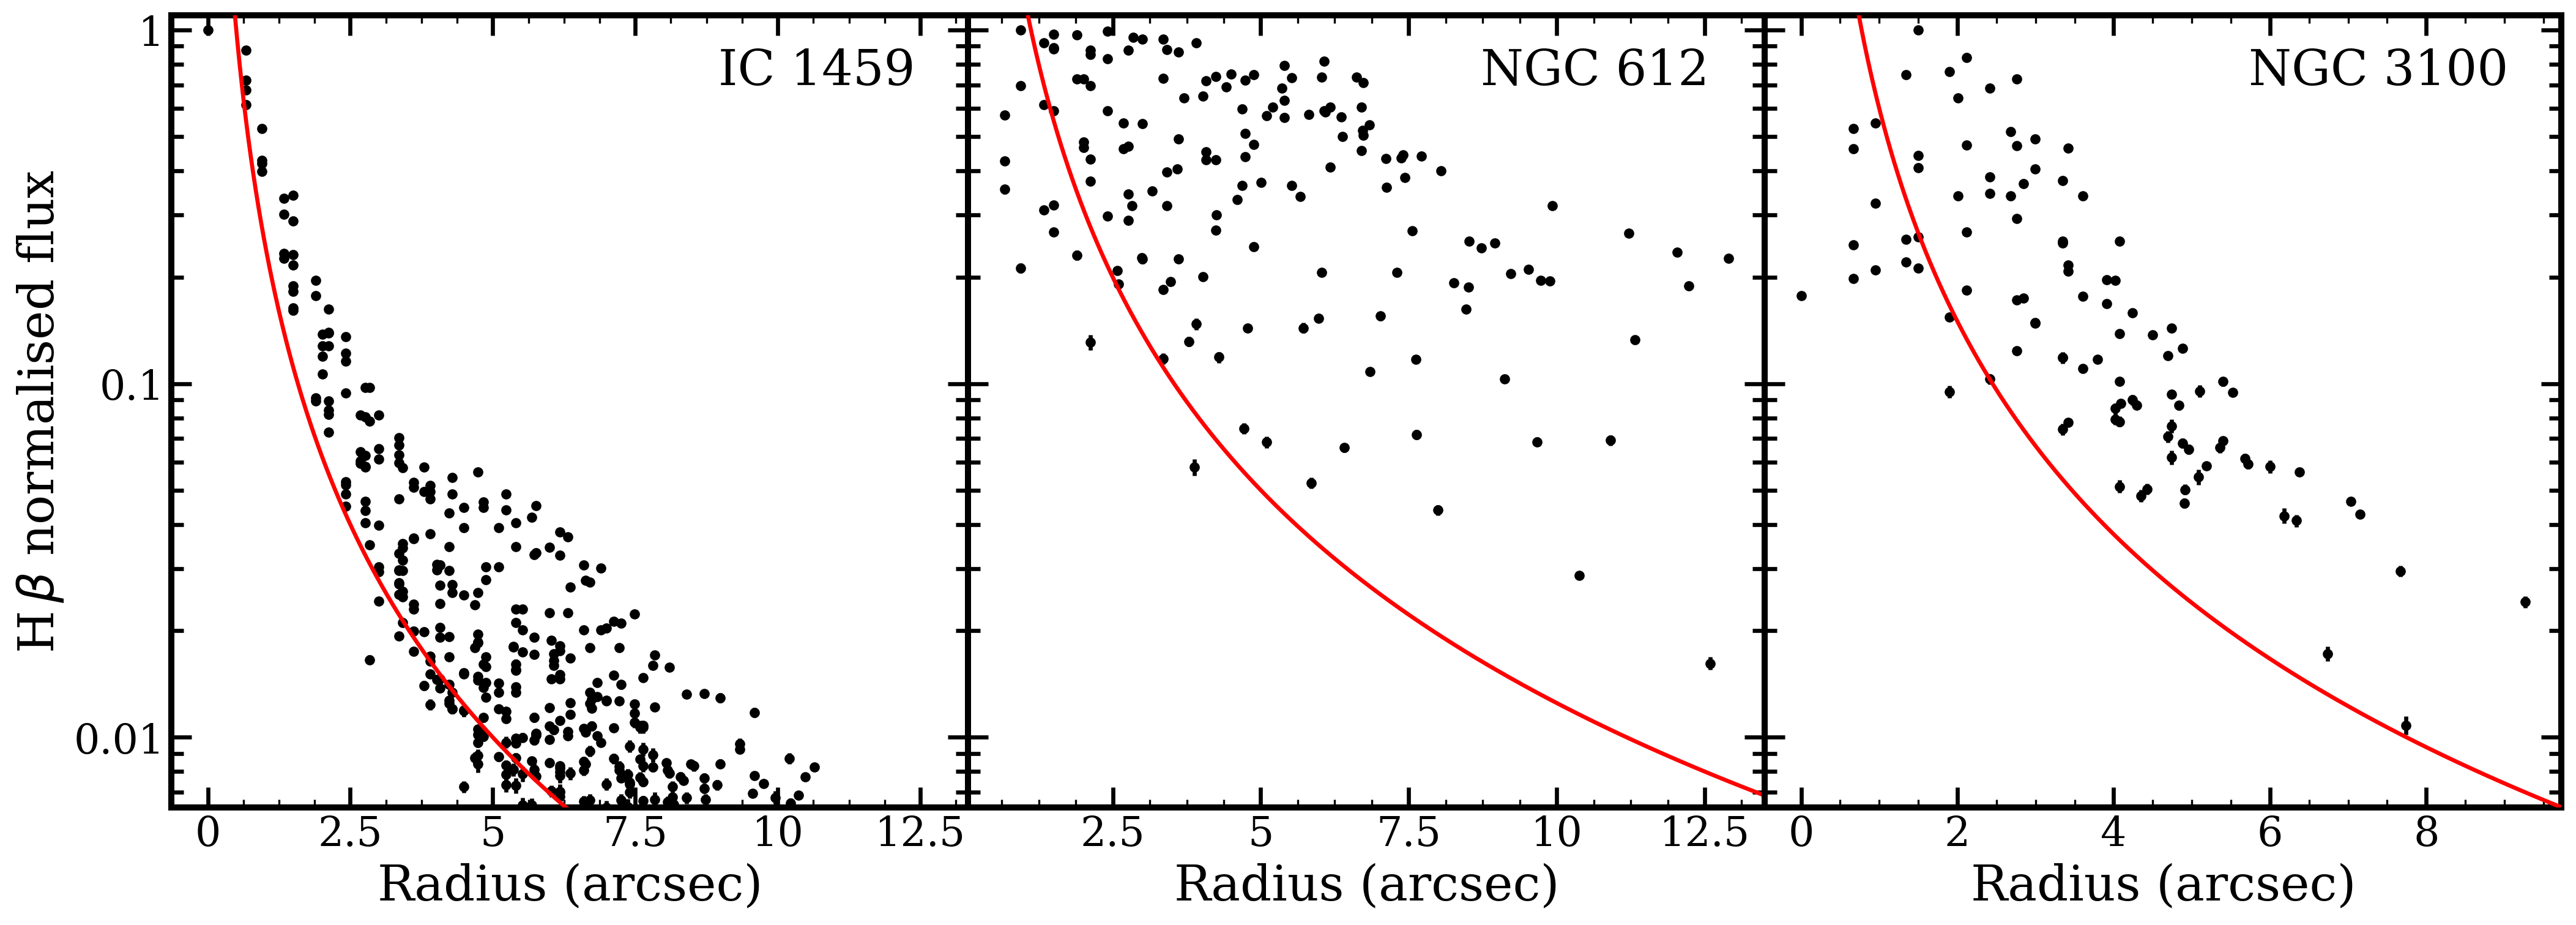
\includegraphics[width=\columnwidth]{Hbeta_profile.png}
				\caption{H$\beta$ flux radial profiles derived from the VIMOS datacubes. Solid red lines show $F(\mathrm{H\beta}) \propto r^{-2}$.}
				\label{fig:Hb_profile_VIMOS}
			\end{figure}

			\begin{figure}
				\centering
				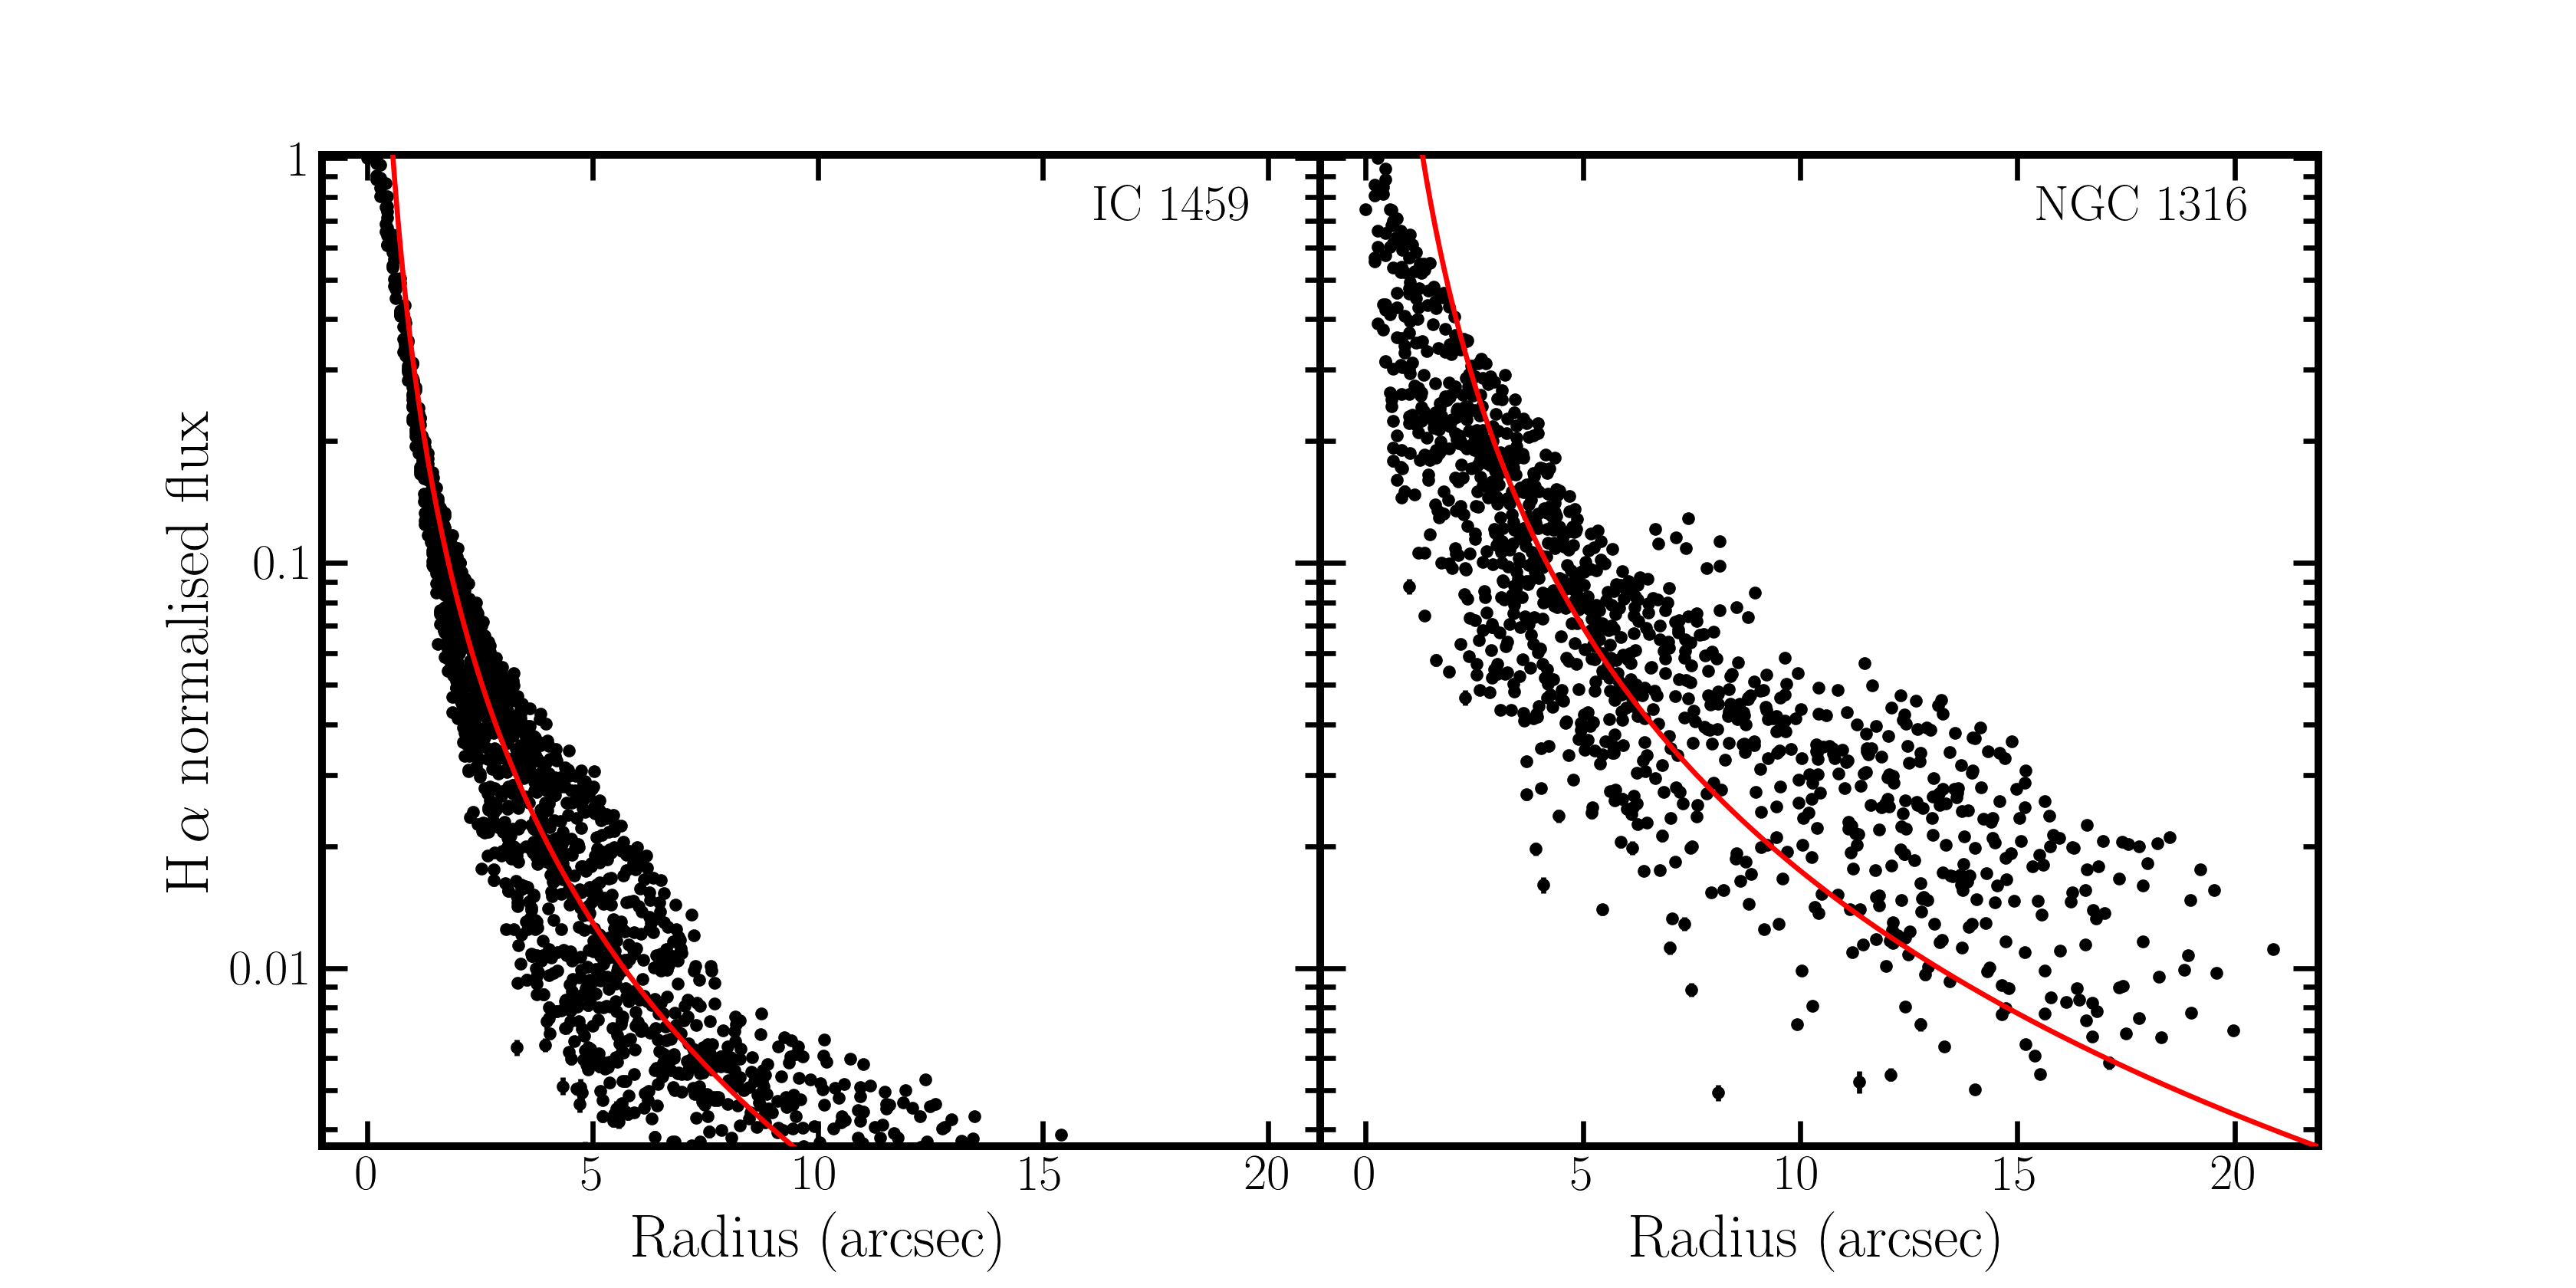
\includegraphics[width=0.73\columnwidth]{Halpha_profile.png}
				\caption{H$\alpha$ flux radial profiles derived from the MUSE datacubes. Solid red lines show $F(\mathrm{H\alpha}) \propto r^{-2}$.}
				\label{fig:Ha_profile_MUSE}
			\end{figure}
			
			As discussed above, many galaxies classified as LINERs are in fact LIERs \citep[see e.g.][]{Sarzi2005, Sarzi2010, Singh2013, Belfiore2016}, i.e.\ the source of the ionizing radiation is not concentrated in the nuclear regions of the galaxies. To check if the ionizing radiation is entirely due to an AGN throughout the host galaxy, we plot the H$\alpha$ and H$\beta$ flux radial profiles for the MUSE and VIMOS data in Figs.\,\ref{fig:Ha_profile_MUSE} and \ref{fig:Hb_profile_VIMOS}, respectively. A point source, such as an AGN, will result in a profile having a $r^{-2}$ shape, where $r$ is the distance of the bin from the galaxy centre. A shallower profile points to a spatially-extended source, presumably non-circumnuclear stellar processes such as star formation or radiation from pAGB stars, as the dominant cause of the ionization in the outer parts of the galaxy (i.e.\ LIER rather than LINER). All the galaxies with spatially-extended Balmer emission in our Southern Sample revel a central point source as the dominant source of the ionizing photons. The H$\beta$ profile of NGC 612 has a larger scatter suggesting that stellar processes also have some impact (likely radiation from pAGB stars, as these galaxies are ETGs and therefore likely have low star-formation rates).

			


		\subsubsection{MEx Diagnostic Plots}
			\label{subsubsec:MEx}
			\begin{figure}
				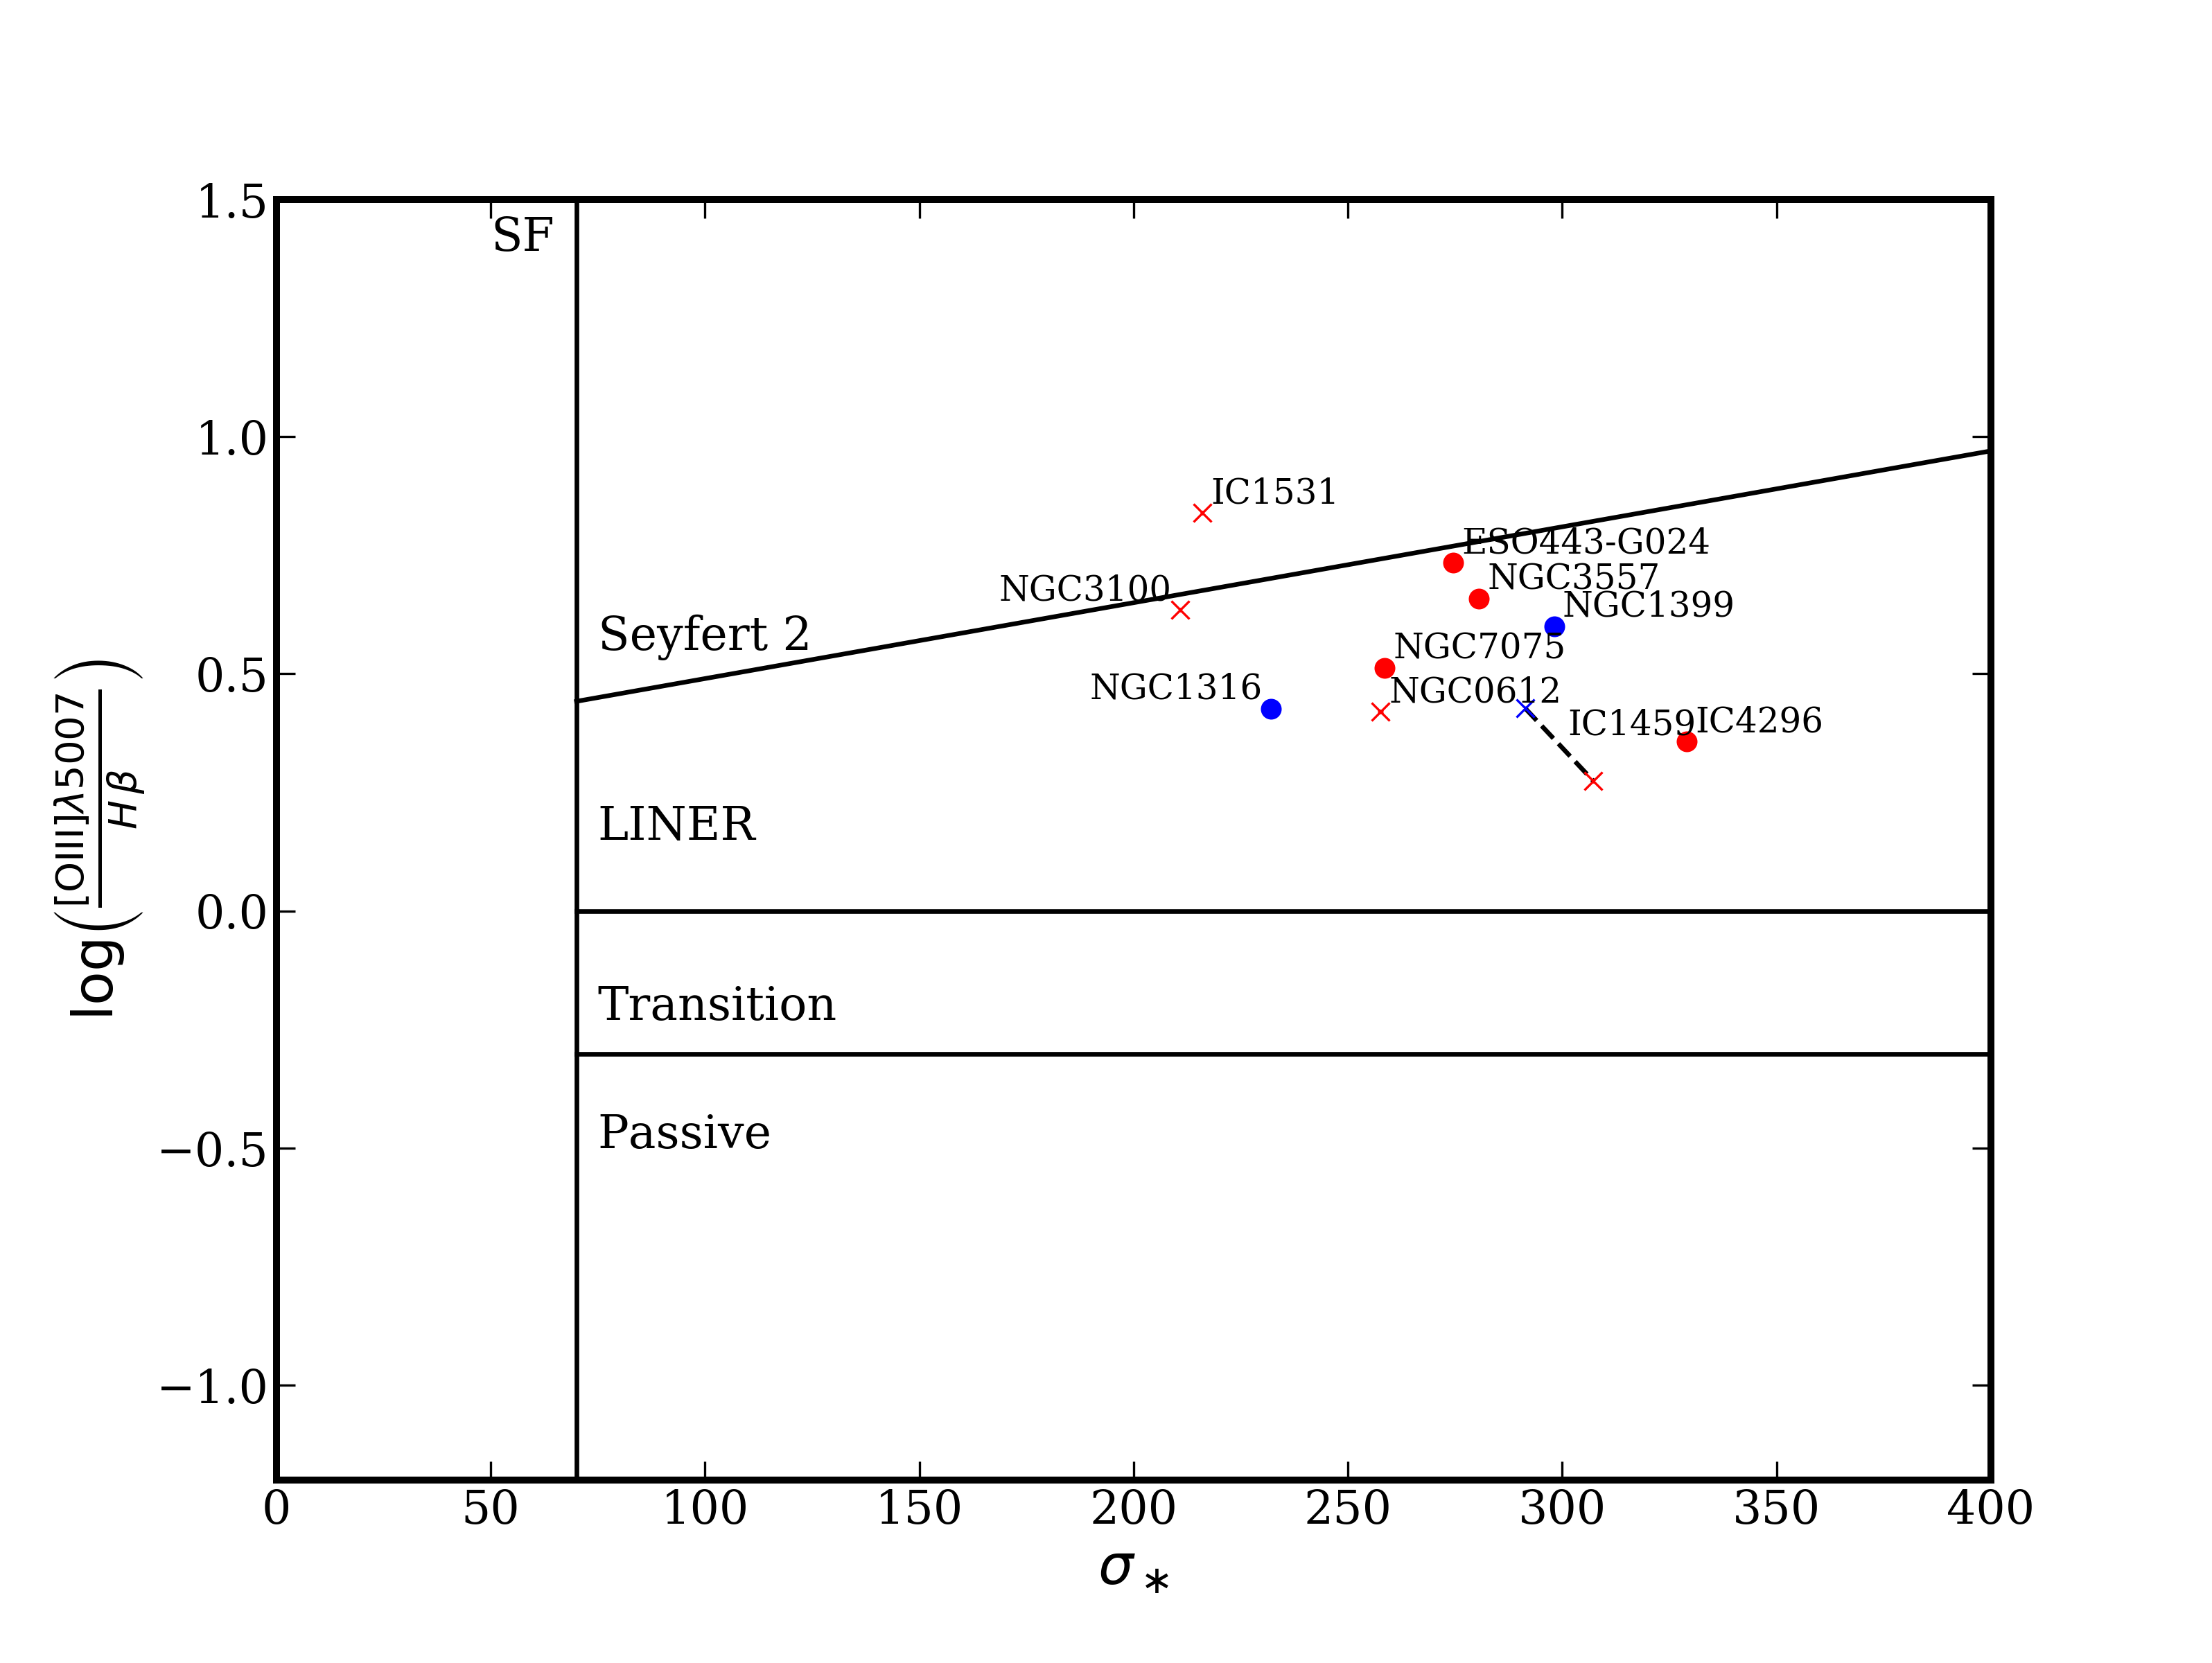
\includegraphics[width=\columnwidth]{nuclear_MEx.png}
				\caption{Nuclear MEx plot, allowing to classify the sources of the ionizing radiation within the central 3\arcsec. Data points derived from the VIMOS and MUSE datacubes are in red and blue, respectively. Crosses mark galaxies with [\ion{O}{iii}]$\lambda$5007 equivalent width $> 0.8$\,\AA, while filled circles show galaxies with [\ion{O}{iii}]$\lambda$5007 equivalent width $\leqslant 0.8$\,\AA. The VIMOS and MUSE data points of IC 1459 are linked with a black dashed line. Classification boundaries are from \citet{Nyland2016}.}
				\label{fig:MEx}
			\end{figure}

			The mass\,--\,excitation (MEx) plot of \citet{Juneau2011} is useful to classify galaxies with intermediate excitation levels ($0.5 < \mathrm{[\ion{O}{iii}]/H\beta} < 8.0$), particularly as it does not depend on faint lines such as the [\ion{N}{I}] doublet. We use here the calibrations by \citet{Nyland2016}, including an attempt to separate LINERs powered by AGN from those powered by pAGB stars (the former have [\ion{O}{iii}] equivalent widths $>0.8$\,\AA). We use an aperture of 3\arcsec\ to plot the nuclear MEx for our Southern Sample galaxies, and the resulting diagnostic plot is shown in Fig.\,\ref{fig:MEx}. 


\section{Discussion and Conclusions}
	\label{sec:discuss}
	In Sections \ref{sec:StarKine} we show that in terms of the stellar kinematic properties, our radio-selected Southern sample are no different to ordinary optically-selected ETGs. Our sample shows a mixture of of regularly- and non-regularly-rotating behaviours, with both classes showing evidence of consistency with observations of the intrinsic shapes of ordinary regular and non-regular rotators. At this stage we observe that two (with a tentative third) galaxies host large KDCs. We also classify our sample galaxies into fast- and slow-rotators and find a consistent fraction ($45\pm13$\%) of slow-rotators to the ordinary ETG samples of the A+M sample, once the difference in the mass distribution between our Southern sample and the A+M sample are taken into account.

	Radio-loud lenticular (S0) galaxies are extremely rare with only a handful of known cases \citep[e.g.][]{Heckman1982, Morganti2011}, presumably due to the associated mass functions of both S0s and radio galaxies: both massive S0s and low-mass radio galaxies are rare, with a similar transition masses from rare to more numerous. NGC 612 is one of those rare cases.

	In terms of absorption line strengths and stellar populations (Section \ref{sec:absorption} and \ref{sec:stellarPop}), we find a remarkably similar gradient to the central Mg\,b verse stellar velocity dispersion relation to that of \citet{Ziegler1997}. Most of the galaxies in our Southern sample show typical ETG behavior: old, metal rich stellar populations, with a few exceptions: NGC 612 and NGC 1316 are both significantly younger than most ETGs and NGC 3557 has a young core. We observe that all 3 KDCs contain old stellar populations and are consistent with being merger remnants. We also show that the KDCs found in Section \ref{sec:StarKine} fit with the age\,--\,size relation found by \citet{Kuntschner2010} (see Section \ref{subsec:popKDC}).

	If molecular (cold) gas is the fuel source that is accreted on to the the central black holes of our Southern sample in order to power the radio jets, unless it is accreted in a highly turbulent fashion, it might be expected that some of that gas might form stars \citep[e.g.][]{Collin1999, Diamond-Stanic2012, LaMassa2013}. If this is the case then a young stellar population might be expected to dominate in the very central (1--2) spaxels. We our best-fitting age maps show no evidence of this. 	

	Section \ref{sec:gas} we show that galaxies in our Southern Sample have ionized gas masses of $10^4$\,--\,$10^6\,\mathrm{M_\odot}$. These are at the upper limit of, and possibly exceed, the typical masses observed in ETGs, although given that our sample contains particularly massive galaxies, high ionized gas masses are not unexpected. 

	The only slow rotator with detected, spatially-extended ionized gas, IC 1459, shows evidence through gas\,--\,star kinematic misalignment that the gas has an external origin, although it is possible that the gas has been re-accreted after it was first ejected during the merger that resulted in the stellar KDC. 

	Of the other 3 galaxies with detected, spatially-extended ionized gas (NGC 612, NGC 1316 and NGC 3100, all fast rotators), we find that one, NGC 3100, again has kinematic evidence of an external gas origin; another, NGC 612, is consistent with an internal origin; while the situation for the last one (NGC 1316) is not clear, although is definitely not in a settled disc. This is in keeping with the findings of \citet{Davis2011a}, who showed that $36\pm5$\% of fast rotators have ionized gas kinematics misaligned with respect to the stellar kinematics, while slow rotators have a flat distribution with respect to their misalignment angles. This indicates that slow rotators are dominated by external sources of gas, while fast rotators can have either internal or external sources. 

	All galaxies with detectable emission lines in our Southern Sample show LINER or Seyfert 2 characteristics. The only Seyfert 2 in our sample is the fast rotator, IC 1531. This is consistent with the results of \citet{Nyland2016}, who showed that all ETGs in the Atlas$^\text{3D}$ sample classified as Seyferts are also fast rotators. We find 9 of the 11 galaxies to be LINERs, 5 of which we conclusively attribute the ionizing photons to the central AGN. The final galaxy, PKS 718-34 has no emission line detections (i.e.\ passive). 

	Overall, we thus find that the warm ISM properties of our Southern Sample galaxies are consistent with those of other jet-mode AGN. These are ordinary ETGs experiencing an active phase, presumably due to the central black holes currently accreting gas in some form. 

	All these observations and findings, are consistent with those of typical massive ETGs. This is consistent with the hypothesis that radio-galaxies are ordinary massive ETGs experiencing a normal but short-lived active phase. 


% \section{Summary}
% 	\label{sec:sum}
% 	In the paper we present VIMOS and archival MUSE IFS observations of 11 low-powered radio galaxies. We find the best-fitting stellar kinematics and populations, as well as find the ionized gas spatial distribution, kinematics and dominant ionizing radiation source. We classify the kinematic maps according to the fast/slow rotator classification scheme of \citet{Cappellari2016} and find a consistent fraction of slow rotators for the mass distribution of our sample. 


\section*{Acknowledgements}

The Acknowledgements section is not numbered. Here you can thank helpful
colleagues, acknowledge funding agencies, telescopes and facilities used etc.
Try to keep it short.

%%%%%%%%%%%%%%%%%%%%%%%%%%%%%%%%%%%%%%%%%%%%%%%%%%

%%%%%%%%%%%%%%%%%%%% REFERENCES %%%%%%%%%%%%%%%%%%

% The best way to enter references is to use BibTeX:

\bibliographystyle{mnras}
\bibliography{refs} % if your bibtex file is called example.bib


%%%%%%%%%%%%%%%%%%%%%%%%%%%%%%%%%%%%%%%%%%%%%%%%%%

%%%%%%%%%%%%%%%%% APPENDICES %%%%%%%%%%%%%%%%%%%%%

\appendix
\section{Maps}
	\label{sec:Maps}

	Here, we present spatially-resolved maps of our Southern Sample of the parameters measured and fitted to the IFS datacubes using the methods described in Section \ref{sec:analysis}. We present each galaxy in turn.

	\subsection{ESO\,443-G24}
		\begin{figure*}
			\centering
			\includegraphics[width=\textwidth]{eso443-g024.png}
			\caption{}
			\label{fig:eso443}
		\end{figure*}

	\subsection{IC\,1459}
		\begin{figure*}
			\centering
			\includegraphics[width=\textwidth]{ic1459.png}
			\caption{As Fig.\,\ref{fig:eso443}, but for IC\,1459}
			% \label{fig:}
		\end{figure*}

	\subsection{IC\,1531}
		\begin{figure*}
			\centering
			\includegraphics[width=\textwidth]{ic1531.png}
			\caption{As Fig.\,\ref{fig:eso443}, but for IC\,1531}
			% \label{fig:}
		\end{figure*}

	\subsection{IC\,4296}
		\begin{figure*}
			\centering
			\includegraphics[width=\textwidth]{ic4296.png}
			\caption{As Fig.\,\ref{fig:eso443}, but for IC\,4296}
			% \label{fig:}
		\end{figure*}

	\subsection{NGC\,612}
		\begin{figure*}
			\centering
			\includegraphics[width=\textwidth]{ngc0612.png}
			\caption{As Fig.\,\ref{fig:eso443}, but for NGC\,612}
			% \label{fig:}
		\end{figure*}

	\subsection{NGC\,1316}
		\begin{figure*}
			\centering
			\includegraphics[width=\textwidth]{ngc1316.png}
			\caption{As Fig.\,\ref{fig:eso443}, but for NGC\,1316}
			% \label{fig:}
		\end{figure*}

	\subsection{NGC\,1399}
		\begin{figure*}
			\centering
			\includegraphics[width=\textwidth]{ngc1399.png}
			\caption{As Fig.\,\ref{fig:eso443}, but for NGC\,1399}
			% \label{fig:}
		\end{figure*}

	\subsection{NGC\,3100}
		\begin{figure*}
			\centering
			\includegraphics[width=\textwidth]{ngc3100.png}
			\caption{As Fig.\,\ref{fig:eso443}, but for NGC\,3100}
			% \label{fig:}
		\end{figure*}

	\subsection{NGC\,3557}
		\begin{figure*}
			\centering
			\includegraphics[width=\textwidth]{ngc3557.png}
			\caption{As Fig.\,\ref{fig:eso443}, but for NGC\,3557}
			% \label{fig:}
		\end{figure*}

	\subsection{NGC\,7075}
		\begin{figure*}
			\centering
			\includegraphics[width=\textwidth]{ngc7075.png}
			\caption{As Fig.\,\ref{fig:eso443}, but for NGC\,7075}
			% \label{fig:}
		\end{figure*}

	\subsection{PKS\,718-34}
		\begin{figure*}
			\centering
			\includegraphics[width=\textwidth]{pks0718-34.png}
			\caption{As Fig.\,\ref{fig:eso443}, but for NGC\,718-34}
			% \label{fig:}
		\end{figure*}





\section{Extrapolating VIMOS Data}
	\label{sec:Decrement}
	\begin{figure}
		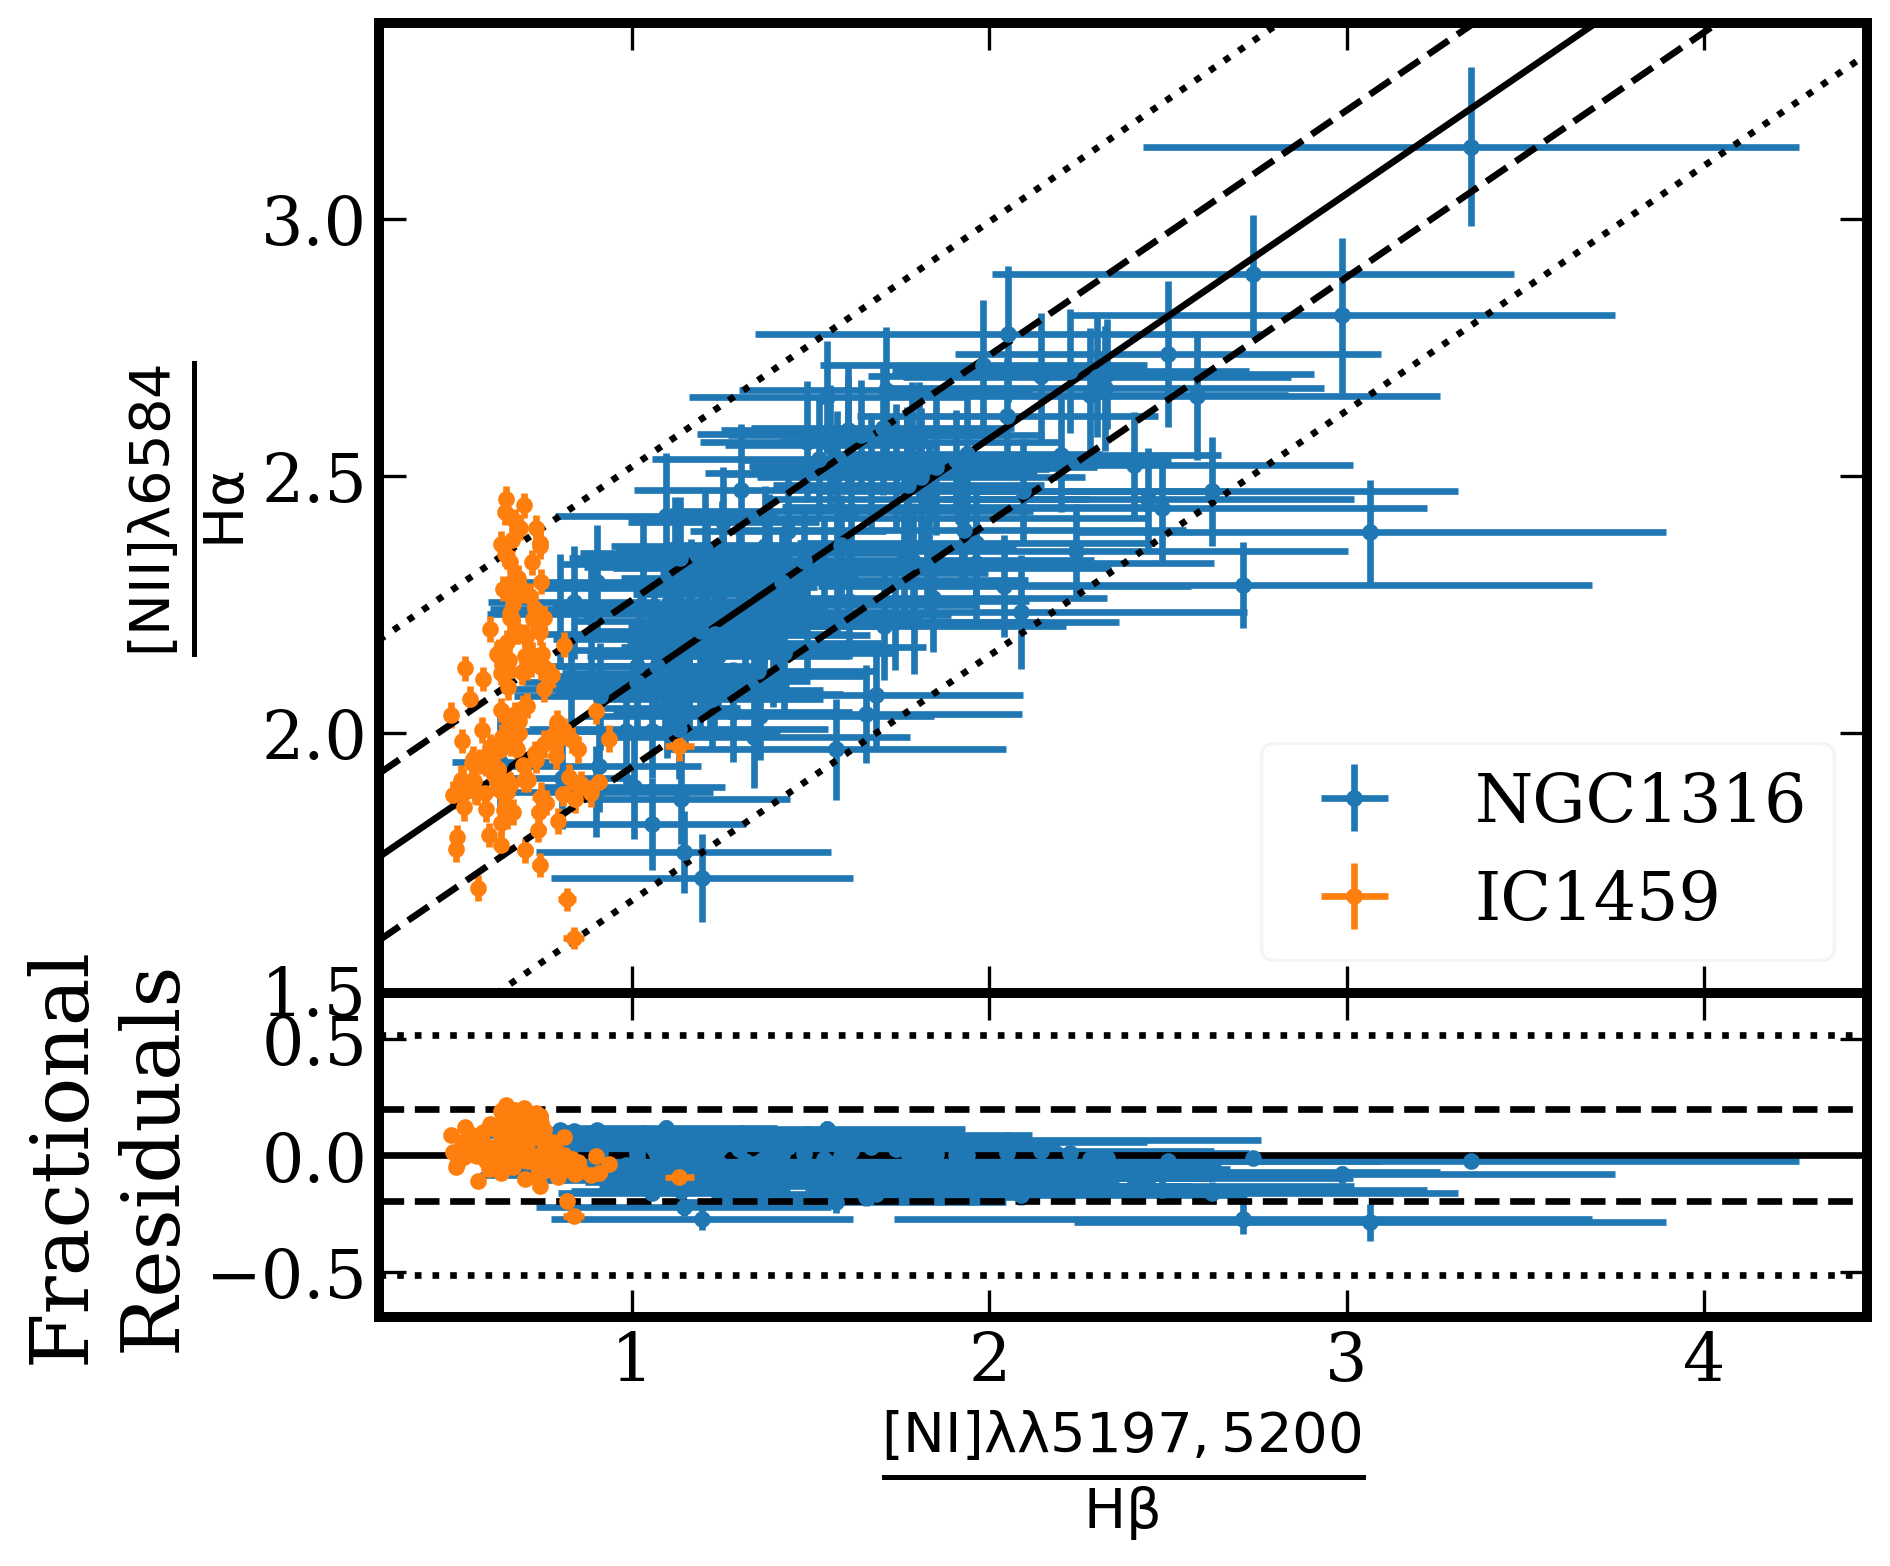
\includegraphics[width=\columnwidth]{ratio_fit.png}
		\caption[\bracket{\ion{N}{ii}}/H$\alpha$ vs \bracket{\ion{N}{i}}/H$\beta$]{Upper panel: [\ion{N}{ii}]/H$\alpha$ vs [\ion{N}{i}]/H$\beta$ line ratios for the galaxies IC 1459 and NGC 1316, used to transform the classification boundaries e.g.\ the classic [\ion{N}{ii}] BPT plot to the SARUON diagnostic plot. Lower panel: Residuals = ([\ion{N}{ii}]/H$\alpha$ - best-fit)/[\ion{N}{i}]/H$\beta$. The solid line shows the best-fitting (Eq.\ \ref{eq:N_dec}) in both panels, while the dashed and dotted lines show the 68 and 99 percentiles, respectively.}
		\label{fig:ratio_relation}
	\end{figure}

	\begin{figure}
		\includegraphics[width=\columnwidth]{EQw_fit.png}
		\caption[Comparing H$\alpha$ and H$\beta$ equivalent widths]{Upper panel: H$\alpha$ vs H$\beta$ equivalent widths for the galaxies IC 1459 and NGC 1316 used to transform the classification boundaries of diagnostics involving the H$\alpha$ equivalent width to those involving H$\beta$. Lower panel: Residuals = (EW(H$\alpha$) - best-fit)/EW(H$\beta$). The solid line shows the best-fitting (Eq.\ \ref{eq:EqW_dec}) in both panels, while the dashed and dotted lines show the 68 and 99 percentiles, respectively.}
		\label{fig:EqW_relation}
	\end{figure}

	% The Balmer decrement, $d_\mathrm{H}$, is the ratio of the H$\alpha$ to H$\beta$ fluxes. There are good theoretical motivations for this ratio to be near constant at $d_\mathrm{H} = 2.86$, under a wide variety of conditions. In reality, however, higher values are routinely observed. These can be explained as due to either the presence of dust causing extinction (whereby emission lines at shorter wavelengths appear dimmer than expected from their redder counterparts due to dust preferentially scattering and absorbing bluer light) or some mechanism that populates hydrogen levels from the ground up. Such mechanisms may be important in high-density environments, such as within powerful (type 1) AGN \citep[e.g.][]{Shields1974, Netzer1975}. 
	%
	% The majority ($\approx 60$\%) of ETGs and all LINER and Seyfert galaxies are dusty \citep[e.g.][]{Martini2013}. 
	% Such galaxies reveal clear dust lanes in \textit{Hubble Space Telescope (HST)} observations \citep[e.g.][]{Martini2013}, are bright in the infrared (where the thermal emission from dust is seen as a dust ``bump''; e.g.\ \citealt{Jura1987, Knapp1992}), and possess other emission lines \citep[e.g.\ \bracket{\ion{S}{ii}};][]{Wampler1968} showing similar reddening. Thus, assuming the observed steepening of the Balmer decrement is entirely due to dust, the ratio of the observed decrement to the theoretical value of 2.86 is a good estimate of the dust reddening.

	If we assume that different ionization states of a given atomic species occur in the same spatial location, then shielding is not important or at least is linear in its effect on the emission-line ratios. Given that the different states are then produced under the same conditions, it is natural to expect a simple relationship between their emission line fluxes, similar to the Balmer decrement. We exploit such relationships to transform classification boundaries from diagnostic plots which use emission lines outside of the spectral range of VIMOS to diagnostics which can be measured with our VIMOS data e.g.\ transform from the classic BPT [\ion{N}{ii}]/H$\alpha$ versus [\ion{O}{iii}]/H$\beta$ to [\ion{N}{i}]/H$\beta$ versus [\ion{O}{iii}]/H$\beta$ diagnostic plot (hereafter the SAURON diagnostic plot) of \citet{Sarzi2010}. We achieve this by finding a best-fitting relationship between the relevant measurements taken in each bin of the galaxies for which we have the relevant detections in our MUSE data (due to the lack of detectable emission line in the observations of IC 4296 and NGC 1399, we therefore use the observations of IC 1459 and NGC 1316). This relationship is then applied to the diagnostic boundary lines in the relevant plots below. We emphasize that these are purely empirical relationships and thus differ substantially from the Balmer decrement with its strong theoretical basis (although these relationships include the effect of the Balmer decrement). 

	The two transformations that we use are from [\ion{N}{ii}]/H$\alpha$ to [\ion{N}{i}]/H$\beta$ line ratios and from the H$\alpha$ to the H$\beta$ equivalent widths. In both cases we fit a linear relationship $y = Ax + B$ using the least-trimmed squares routine, \textsc{lts\_linefit}\footnote{http://www-astro.physics.ox.ac.uk/\~mxc/software/\#lts} of \citet{Cappellari2013} due to its robust handling of the uncertainties along both axes. These are shown in Figs.\ \ref{fig:ratio_relation} and \ref{fig:EqW_relation}, where we find
	\begin{equation}
		\frac{[\text{\ion{N}{ii}}]}{H\alpha} = \, (0.38 \pm 0.02) \frac{[\text{\ion{N}{i}}]}{H\beta} + (1.80 \pm 0.02)
	\end{equation}
	and	
	\begin{equation}}
		\mathrm{EW}(H\alpha) = \, (2.92 \pm 0.03) \mathrm{EW}(H\beta) - (0.16 \pm 0.02) \, ,
			\label{eq:EqW_dec}
	\end{equation}
	respectively. Since it is sometimes observed that [\ion{N}{ii}]/H$\alpha < 1.80$, which if blindly applying the relationship found above, results in an unphysical [\ion{N}{i}]/H$\beta < 0$ (i.e.\ negative flux), we instead rearrange and use
	\begin{equation}
		\frac{[\text{\ion{N}{i}}]}{H\beta} = \, 
		\begin{cases}
			(0.38 \pm 0.02) \frac{[\text{\ion{N}{iI}}]}{H\alpha} + (1.80 \pm 0.02), & \text{if}\ \frac{[\text{\ion{N}{ii}}]}{H\alpha} < 2 \\
			(0.38 \pm 0.02) \frac{[\text{\ion{N}{ii}}]}{H\alpha}, & \text{otherwise.}
		\end{cases}
		\label{eq:N_dec}
	\end{equation}

%%%%%%%%%%%%%%%%%%%%%%%%%%%%%%%%%%%%%%%%%%%%%%%%%%


% Don't change these lines
\bsp	% typesetting comment
\label{lastpage}
\end{document}

% End of mnras_template.tex